\chapter{\gtest\ descriptions}
\label{chap:gtestdescription}
%For understanding grid electron emission in the \lze\ detector, we designed a gaseous xenon detector to study grid behavior in a similar environment as in the \lze\ detector. We measure electron emission rate from the grid under different grid operating voltages. It helps us figure out the optimal operation voltages for grids in the \lze\ detector. We study different method for reducing electron emission background. Reduction of electron emission background rate from the grid wires will significantly improve our sensitivity to low energy events. This in return will improve our understanding of low mass WIMPs. It will also help to keep the trigger environment in \lze\ quieter. This reduces the systematic errors for S1 and S2 and improve their quality. From that, we will improve our events classification and energy reconstruction. 

%Understanding electron emission processes from the grids in the \lze\ detector, and reducing the rate of this process are essential for the operation of the \lze\ detector. Among all different electron emission processes, 
\lze\ is particularly interested in electric field induced electron emission from the metallic grid. This phenomenon is one of the major sources of background events. Therefore, reduction of the field induced electron emission rate should greatly benefit physics studies in the \lze\ detector.

The electric field induced electron emission events look like low energy events in the \lze\ detector. Thus, reduction of electron emission background rate from the grid wires improves our sensitivity to low energy events. This in return improves our ability to study low mass WIMPs. 

The frequent electron emission events may also accidentally coincidence with the wanted signals, such as S1 and S2, in the \lze\ detector. Reduction of electron emission rate also helps to keep the data recording environment in \lze\ cleaner. This reduces the systematic errors for S1 and S2 and improve their qualities. From that, we improve our events classification and energy reconstruction. This in return improves all physics studies from the \lze\ detector. 

The frequent electron emission events also consume data recording ability in \lze . This may prevent or interrupt recordings of the wanted data. Thus, reduction of electron emission rate also helps to keep the data recording environment in \lze\ quieter to allow longer detector live times for wanted events.
%The maximum operation electric field on the grids in the \lze\ elector set the maximum grids operation voltages. 

Therefore, we develop a two-fold study the reduction of electric field induced electron emission rate in two small detectors. These two detectors are smaller comparing to the \lze\ detector. They are capable of testing a pair of "small" grids. The surface area of these "small" grids are \SI{\sim 1}{\percent} the area of grids that will be used in \lze . 

In the first step, a gaseous detector, below "\gtest ", is built to study different method for reducing electron emission rate. This detector measures electron emission rates on different electric fields before and after different physical and chemical processes. Once this comparison confirms the effects on reduction of the electric field induced electron emission rate, a second stage of study in a liquid xenon detector, below \phaseone , to confirm the reduction persist in liquid xenon environment, which is the environment \lze\ grids operate in. 

%This chapter focus on \gtest .
%This detector measures scintillation and electroluminescence (EL) light signals from events in the detector. This detector operates with gaseous xenon, gaseous argon, and vacuum.  
%We measure electron emission rate from the grid under different grid operating voltages. It helps us figure out the optimal operation voltages for grids in the \lze\ detector. We study different method for reducing electron emission background.
%consist with two major parts: the operation system and data acquisition system. 

%The operation system contains four parts: the tested grids, the gas handling and distribution system, the high voltage system and the light collection system. The gas handling and distribution system is for delivering and storing quality pure gas to the \gtest\ . It includes the operation chamber, the gas circulation panel and plumbing, pressure and temperature sensors of different range, and a separated purity measurement system. The high voltage system includes the power supply, high voltage feed through, cables, and cable termination. The light collection system for measuring the quantity of scintillation light created in the detector includes two PMTs, and the PTFE light reflector.

%The data acquisition(DAQ) system is attached directly onto the output of the two PMTs. It does PMT pulse amplification, shaping, digitizing, transferring and storing.   

%The recorded events were passed to a data processing framework to reduce the dimensions of the input data. Then, the reduced quantity data(RQs) were sent for event classification to select the interesting events. Because of the rate of the electron emission event we are mostly interested in has a various range, in some case really rare. A studying of background events for its the pulse shape, and energy distribution were done to reduce the uncertainty of the emission event rates. And this also helps to give a electron emission selection efficiency. 

%Simultaneously, a light creation and propagation simulation were done for different event classes at different locations to confirm the pulse shape for different event classes.  

%Finally, the knowledge of event classification were used to study the electron emission from different tested grids that we measured.  

%In this chapter, I will first introduce the design concepts of each individual components in detail about \gtest\  that we designed for measuring the electron emissions. Then I will talk about the data acquisition and data processing framework. Then, I will talk about analysis frame work. the light creation and propagation simulations in the detector for the electron emission events. I will discuss characteristic pulse shape and rate of the background events, along with the simulations for these events. Finally, I will discuss the results from different grids from this detector.

This chapter focuses on \gtest . I will first introduce the design concepts of each individual components in \gtest\ . Then I will talk about data acquisition and data processing framework. Then, I will talk about the analysis frame work. This includes event selections , simulations and validations. I will discuss characteristic pulse shape and rate of the background events. Finally, results from these measurements for different grids will be discussed in Chapter.\ref{chap:gtestresult}.

\section{The gaseous detector}
The gaseous detector, \gtest , is designed for studying grid behavior under high voltage for \lze . It measures scintillation and electroluminescence (EL) light signals from events in the detector. Pairs of grids are made with the same material, wire pitch, and wire diameter as the grids that will be used for \lze . The differences between these grids and grids in \lze\ are the diameters of the grid planes. The same pair of grids can also be tested in \phaseone  for studying their performance in liquid xenon. Since these grid are physically similar to \lze\ except for the overall surface area, the results from studying these grids are an useful guidance for \lze\ grid design. 

Grid sparking tests are done on understanding the maximum operation voltage and the optimal operation voltage. Grid sparking tests are performed with both gaseous xenon and argon in various pressures. It is to look for discharges in the detector with biasing the grids. Discharges are discovered with current monitors measuring the short increasing of currents go from the power supply to the grids. A charged-couple device (CCD) camera is used to monitor discharges occur near the EL region. Grid sparking tests provide the detector operation informations for grid emission tests. 

Electron emissions from the grid wires are studied by grid electron emission tests. Grid electron emission tests are usually performed with gaseous xenon at \SI{0.137}{\mole\per\liter} (\SI{\sim 3.3}{\bara} at temperature \SI{295}{\kelvin}). This gas density is noted as standard xenon gas density below. Grid electron emission tests look for \eep\ from grids with PMTs. 

\paragraph{Detector}
The detector operates with xenon gas, argon gas, and vacuum. Operation pressure for this detector is in range \SIrange{e-5}{3.5}{\bara}. 

A cylinder vessel of \SI{10}{\inch} diameter and \SI{24}{\inch} height is used to host electroluminescence detector. Pressure and temperature of the detector are monitored by sensors mounted above the vessel. A gas circulation system is used to add, remove and purify gas for the detector. Fig.~\ref{fig:chambergeneral:vessel} and Fig.~\ref{fig:chambergeneral:gridtest} show the physical layout of the vessel setup and the electroluminescence detector inside. 

The electroluminescence detector (ELD) is the major location of active measurable events. Its conceptual drawing is illustrated in Fig.~\ref{fig:BasicELD}. A pair of grids for measurement are mounted in the center of the vessel. They are separated apart by \SI{13}{\mm} by 12 PEEK spacers. These two grids are biased to different voltages during the measurement. This create an operation voltage difference between the two grids. It enables electrons between these two grids to produce EL photons which can be measured by the PMTs. The region between these two grids is noted as EL region. 

These grids are named after their physical location in the detector as top grid and bottom grid. The grid plane diameters are \SI{140.9}{\mm} for the top grid and \SI{137.4}{\mm} for the bottom grid. Voltages of the two grids are noted as $V_{T}$ for the top grid and $V_{B}$ for the bottom grid. The voltage difference between the top and bottom grid is noted as operation voltage $dV \equiv V_{T} - V_{B}$. They also have another name by their bias voltage. The more anodic grid is called anodic grid. The more cathodic grid is called cathodic grid. Their voltage are also sometimes noted as $V_{A}$ for the anodic grid and $V_{C}$ for the cathodic grid. Normally, the top grid is anodic and the bottom grid is cathodic to study electron emission from the bottom grid. This is normal polarity operation. Occasionally, the top grid is cathodic and bottom grid is anodic to study electron emission from the top grid. This is reverse polarity operation. 

Two PTFE reflector cones are used to improve light collection efficiency for the primary scintillation and EL photons. These reflector cones are mounted on the top and bottom of the EL region. The surface of PTFE cones overhang \SI{0.1}{mm} above the grid. The diameters of the opening of the PTFE cone to the grids are \SI{130}{mm}. Light collection will have the most sensitivity for grid \eep\ in this region. This defines the overall grid surface area of studying. Two PMTs mounted on the PTFE reflector cones are used to measure the primary scintillation and EL photons. Distances between the PMTs to the closest grids are \SI{110.5}{\mm}.

A CAEN R1470ETD high voltage power supply is used to bias the two grids and the two PMTs. Two custom ceramic feed throughs are used to deliver high voltage into the detector vessel to the two grids. Each feed through has a low-pass filter box attached for noise removal. Custom designed cables and cable terminations are used to apply power from the feed throughs to the grids. The cable terminations had limited us biasing grids to high voltage. Improvements of designs are established to solve this problem. Details of iterations of these designs will be discussed in Chapter.~\ref{chap:gtestresult}.    

\begin{figure}[!tb]
\centering
\includegraphics[width=\halfwidth,clip,trim={0 0 0 0},angle=0,origin=c]{Figures/GasTest/WeiDrawEvent/BasicELD.jpg}
\caption[\gtest\ electroluminescence detector]{Conceptual drawing of \gtest\ electroluminescence detector (ELD)}
\label{fig:BasicELD}
\end{figure}

\paragraph{Gas circulation system}
A gas circulation system is used for adding, removing, purifying xenon gas in the detector. The circulation system %panel is designed for continuous purification of noble gas element in the detector. This
also is used to maintain gas purity condition. It removes impurity atoms such as oxygen, water, and hydrocarbons. The purity of xenon gas makes sure that electrons that is created in ELD do not combine with impurity atoms, thus been prevented to produce EL light. The purity of xenon also has an notable effect on electron drift velocity in xenon gas. Impure xenon gas tend to have a slower drift velocity. The deviation of drift velocity between different impurity level can reach \SI{20}{\percent} at certain reduced electric field (ratio of electric field to gas density), as described in Ref.~\ref{Brooks1982}. 

Xenon purification is done through circulating xenon gas through a getter purifier. A gas circulation panel is used to control the flow of xenon gas. A SAES PS3-MT3-R-1 rare gas getter mounted on the circulation panel is used to purify the gas. The getter element has a sub-ppb efficiency of removing water, nitrogen, oxygen, carbon oxide, carbon dioxide, hydrogen, and hydrocarbons%. The capacity of the getter is more than \todo{\SI{0.1}{\meter\cubed}} in volume of nitrogen and oxygen. 
%With continuous purification, noble xenon gas achieves a purity of nitrogen, oxygen and water contamination better than \SI{1}{\ppb}
, as described in Ref.~\cite{SAESgetters2002}.  A custom pump manufactured by KNF Neuberger, Inc. is used to drive the gas circulation in the system. This pump is a type PM26101-0150.1.2.12 double diaphragm pump, which has company specified \SI{1.5}{\bar} operation pressure, as described in Ref.~\cite{KNFNeuberger}. During the actual operation, the pump is working at pressure up to \SI{3.7}{\bar}. The diaphragm pump shows a leak rate less than \SI{e-7}{\bar\liter\per\s}. The circulation flow rate is controlled by a Alicat MC-5SLPM-D-485 \todo{$model number need check$} mass flow controller on the gas circulation panel. It allows a maximum flow rate at \SI{5}{\slpm}, as described in Ref.~\cite{AlicatScientific}. 
Fig.~\ref{fig:chambergeneral:panel} shows the gas circulation panel. 

Two \SI{4}{\liter} bottles are used for the storage of xenon gas used in the tests. These bottles are can be inserted to two dewars. The dewars are filled with liquid nitrogen during removing xenon gas process. Reducing the temperature of the bottle by liquid nitrogen allows xenon to flow back to and condense inside the bottles. During adding xenon gas process, the bottles are taken out from the dewar and warmed up. Fig.~\ref{fig:chambergeneral:bottles} shows the pump and storage bottles for the detector. 

\begin{figure}[!p]
\centering
\begin{subfigure}[b]{\halfwidth}
  	    	\centering
 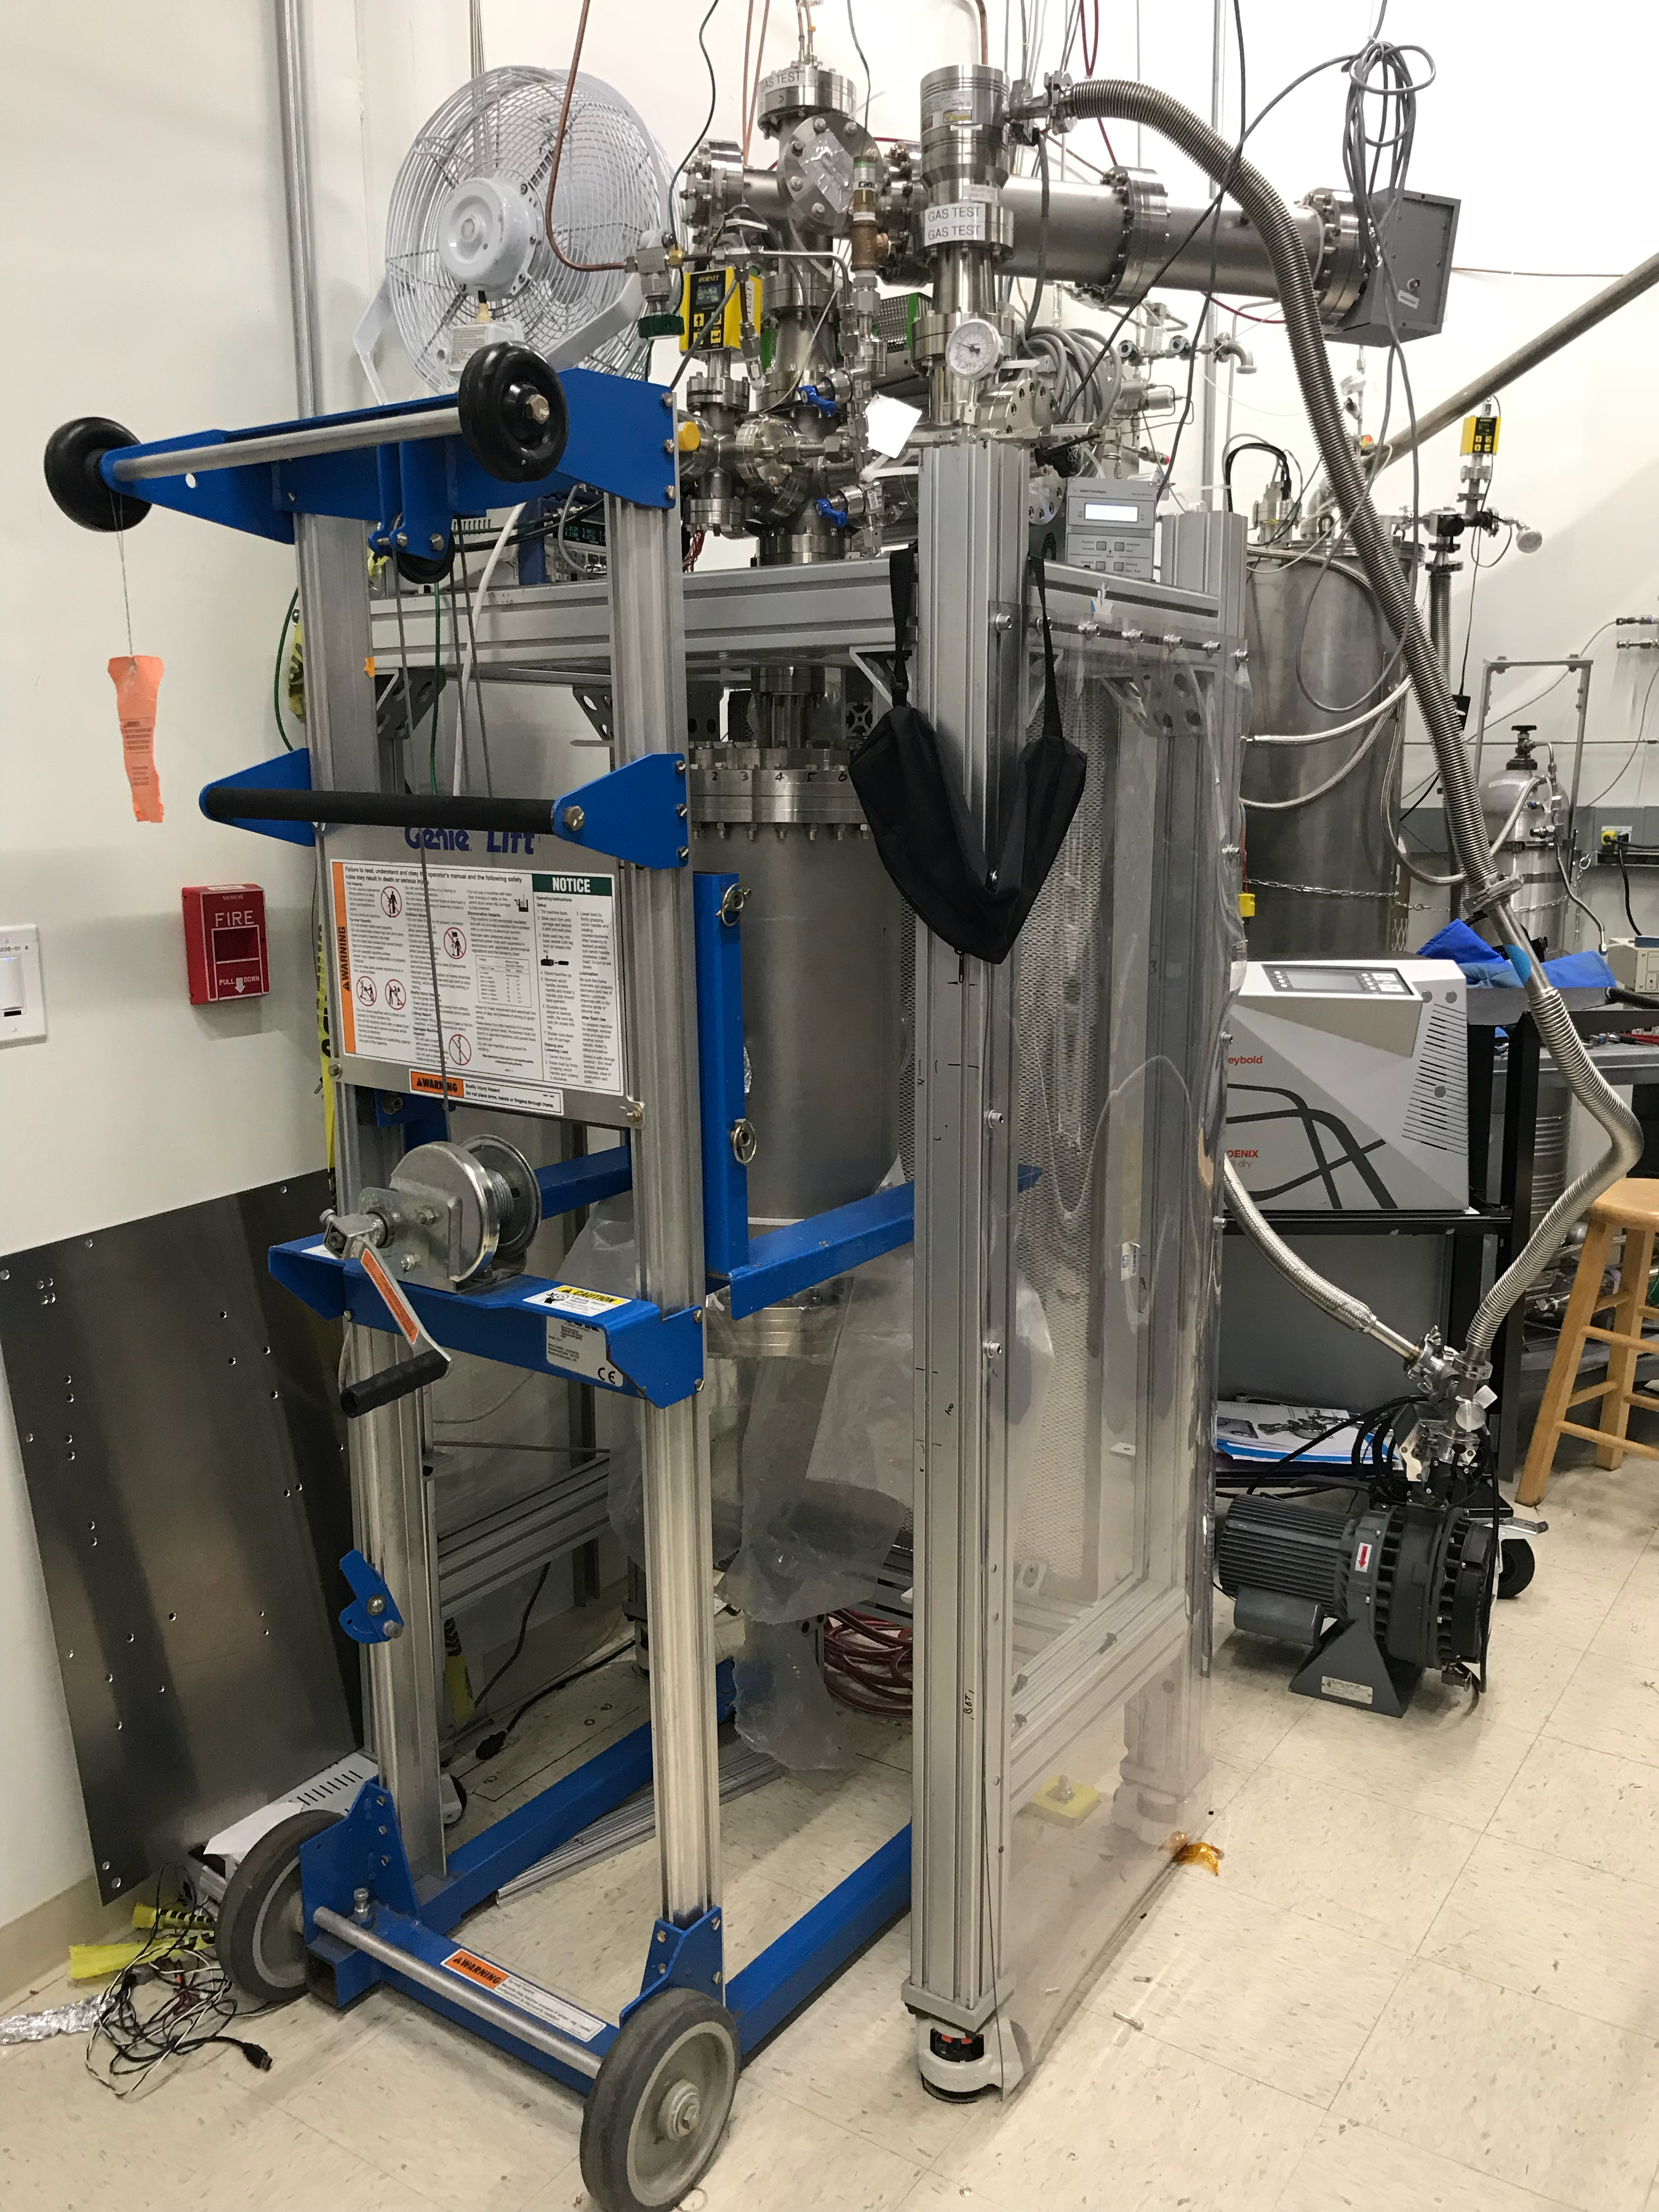
\includegraphics[width=\figurewidth,clip,trim={0 0 0 0},angle=0,origin=c]{Figures/GasTest/PhysicalLayout/GTWholeVessel.jpg}
 \caption{}
 \label{fig:chambergeneral:vessel}
\end{subfigure}
\begin{subfigure}[b]{\halfwidth}
  	    	\centering
 \includegraphics[width=\figurewidth,clip,trim={0 0 0 0},angle=0,origin=c]{Figures/GasTest/PhysicalLayout/GTGridTestRegion.jpg}
 \caption{}
 \label{fig:chambergeneral:gridtest}
\end{subfigure}
\begin{subfigure}[b]{\halfwidth}
  	    	\centering
 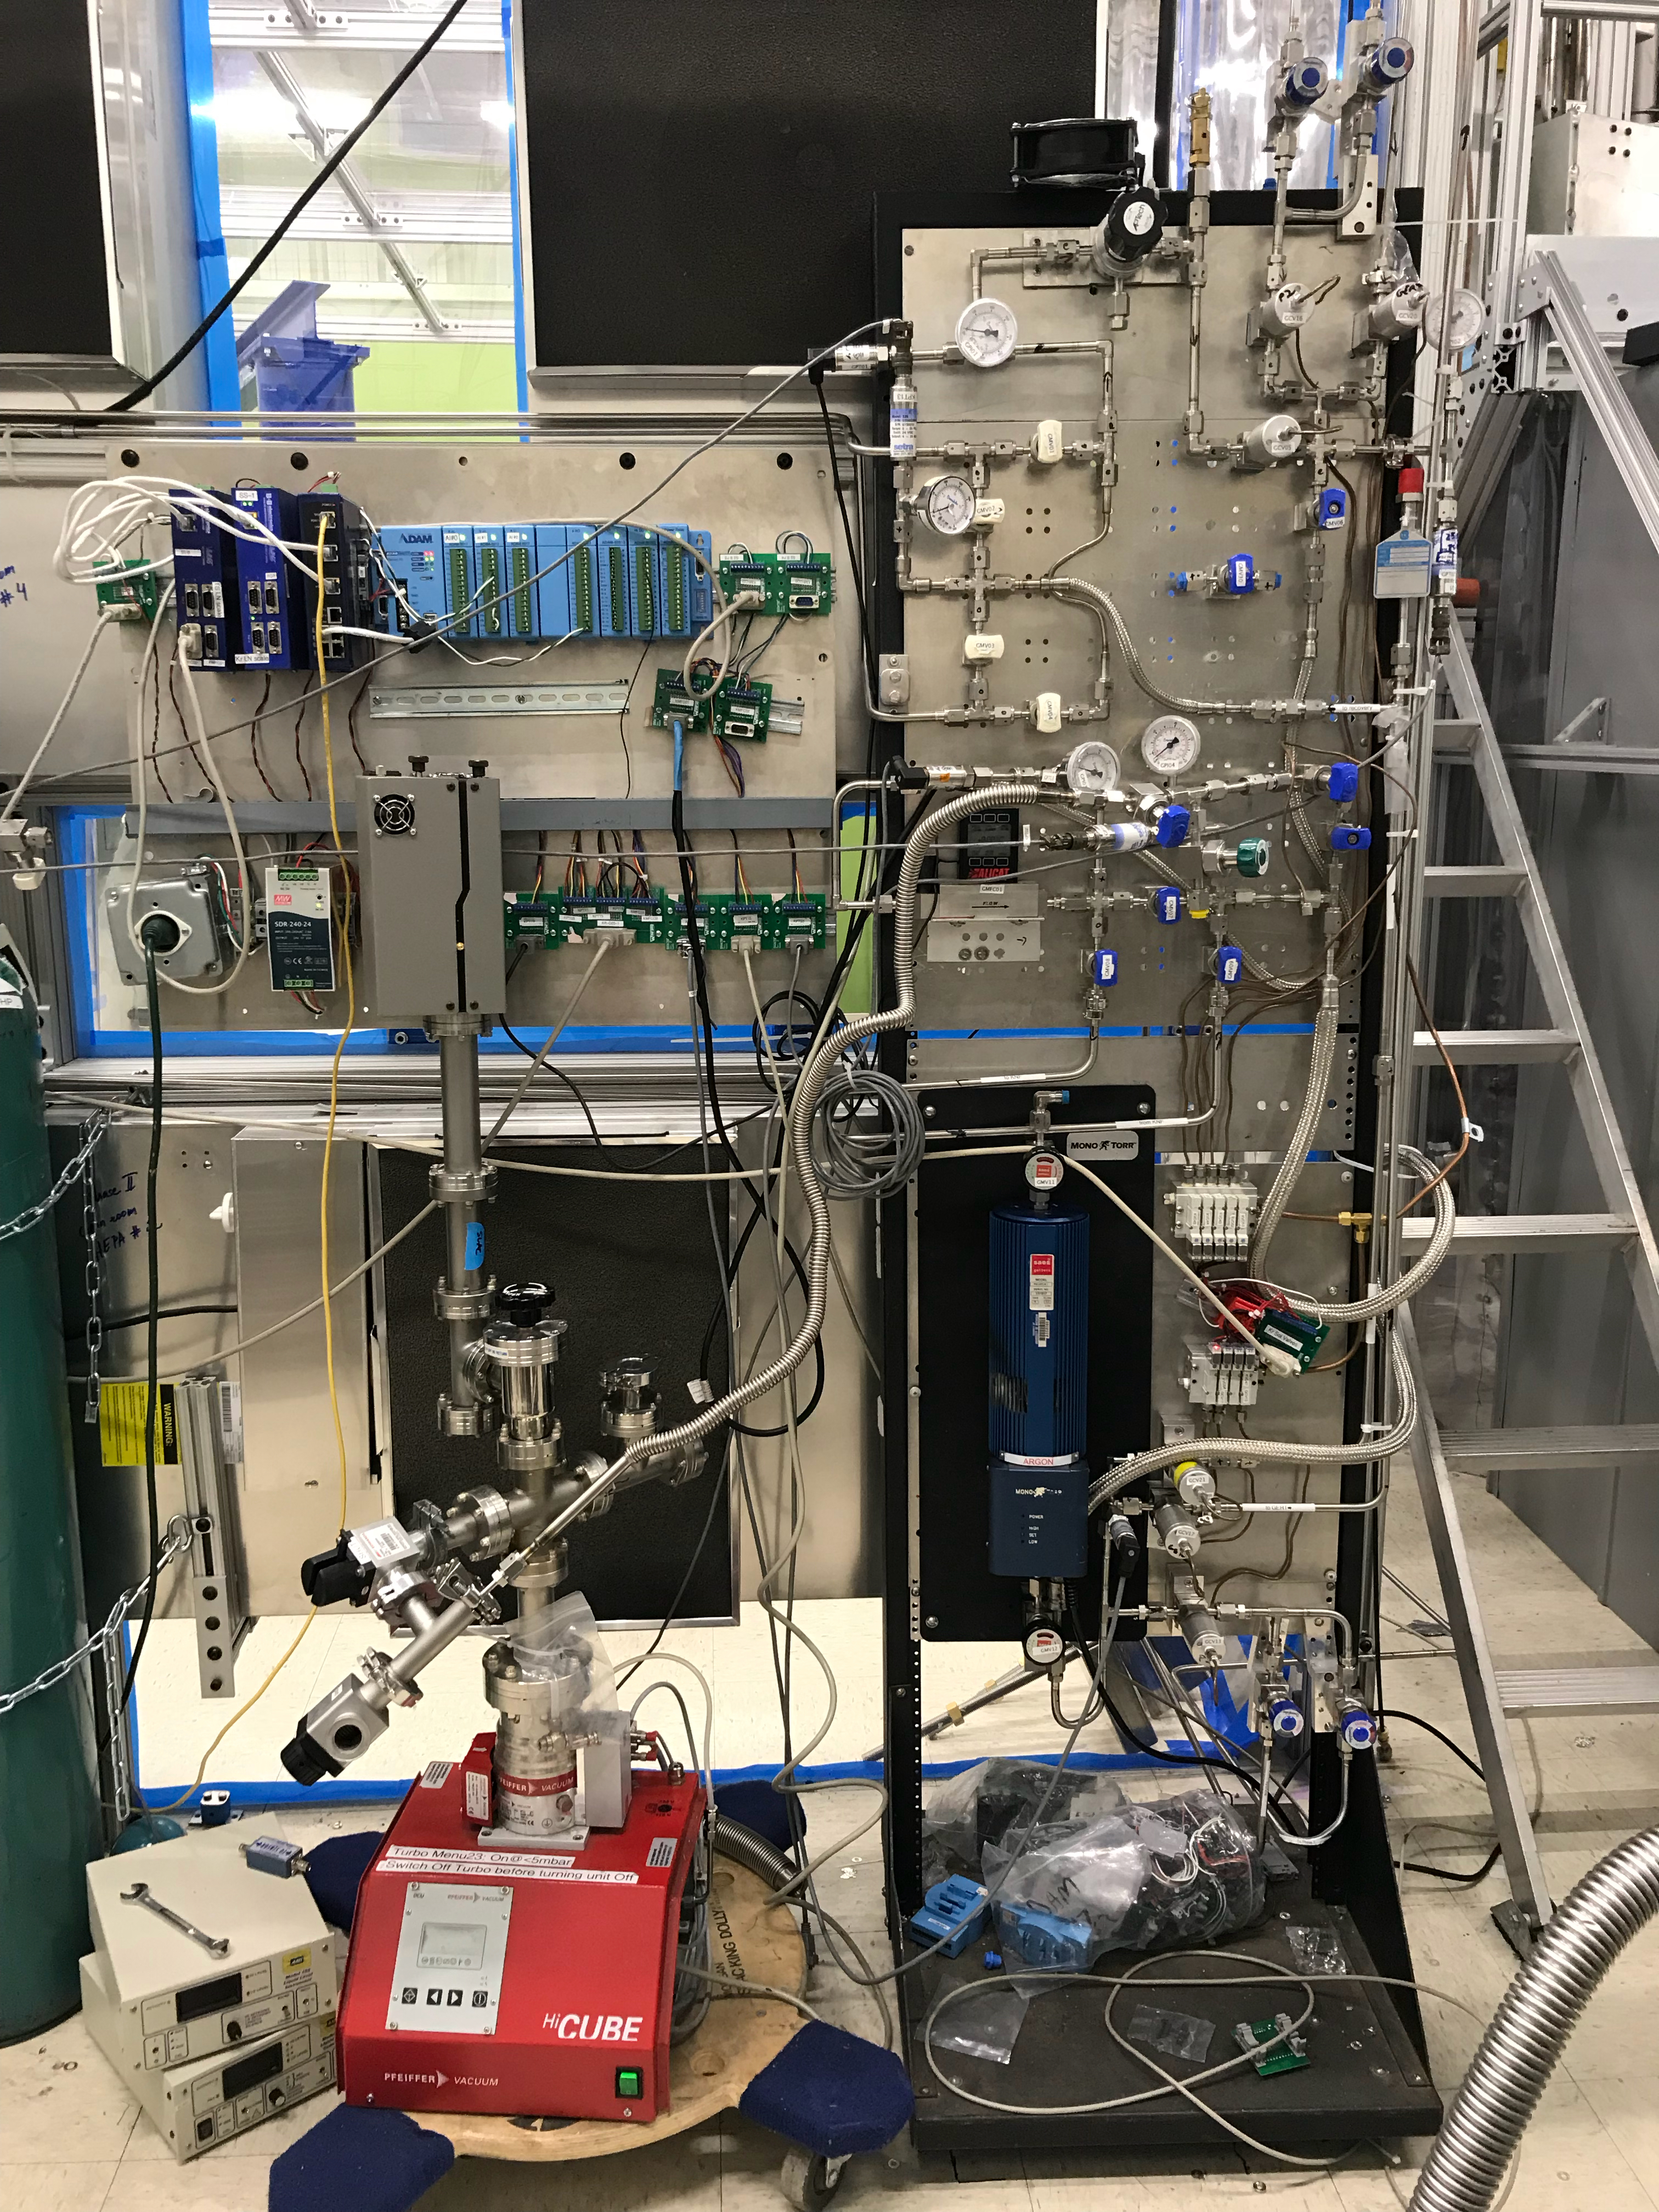
\includegraphics[width=\figurewidth,clip,trim={0 0 0 0},angle=0,origin=c]{Figures/GasTest/PhysicalLayout/GTGasPanel.jpg}
 \caption{}
 \label{fig:chambergeneral:panel}
\end{subfigure}
\begin{subfigure}[b]{\halfwidth}
  	    	\centering
 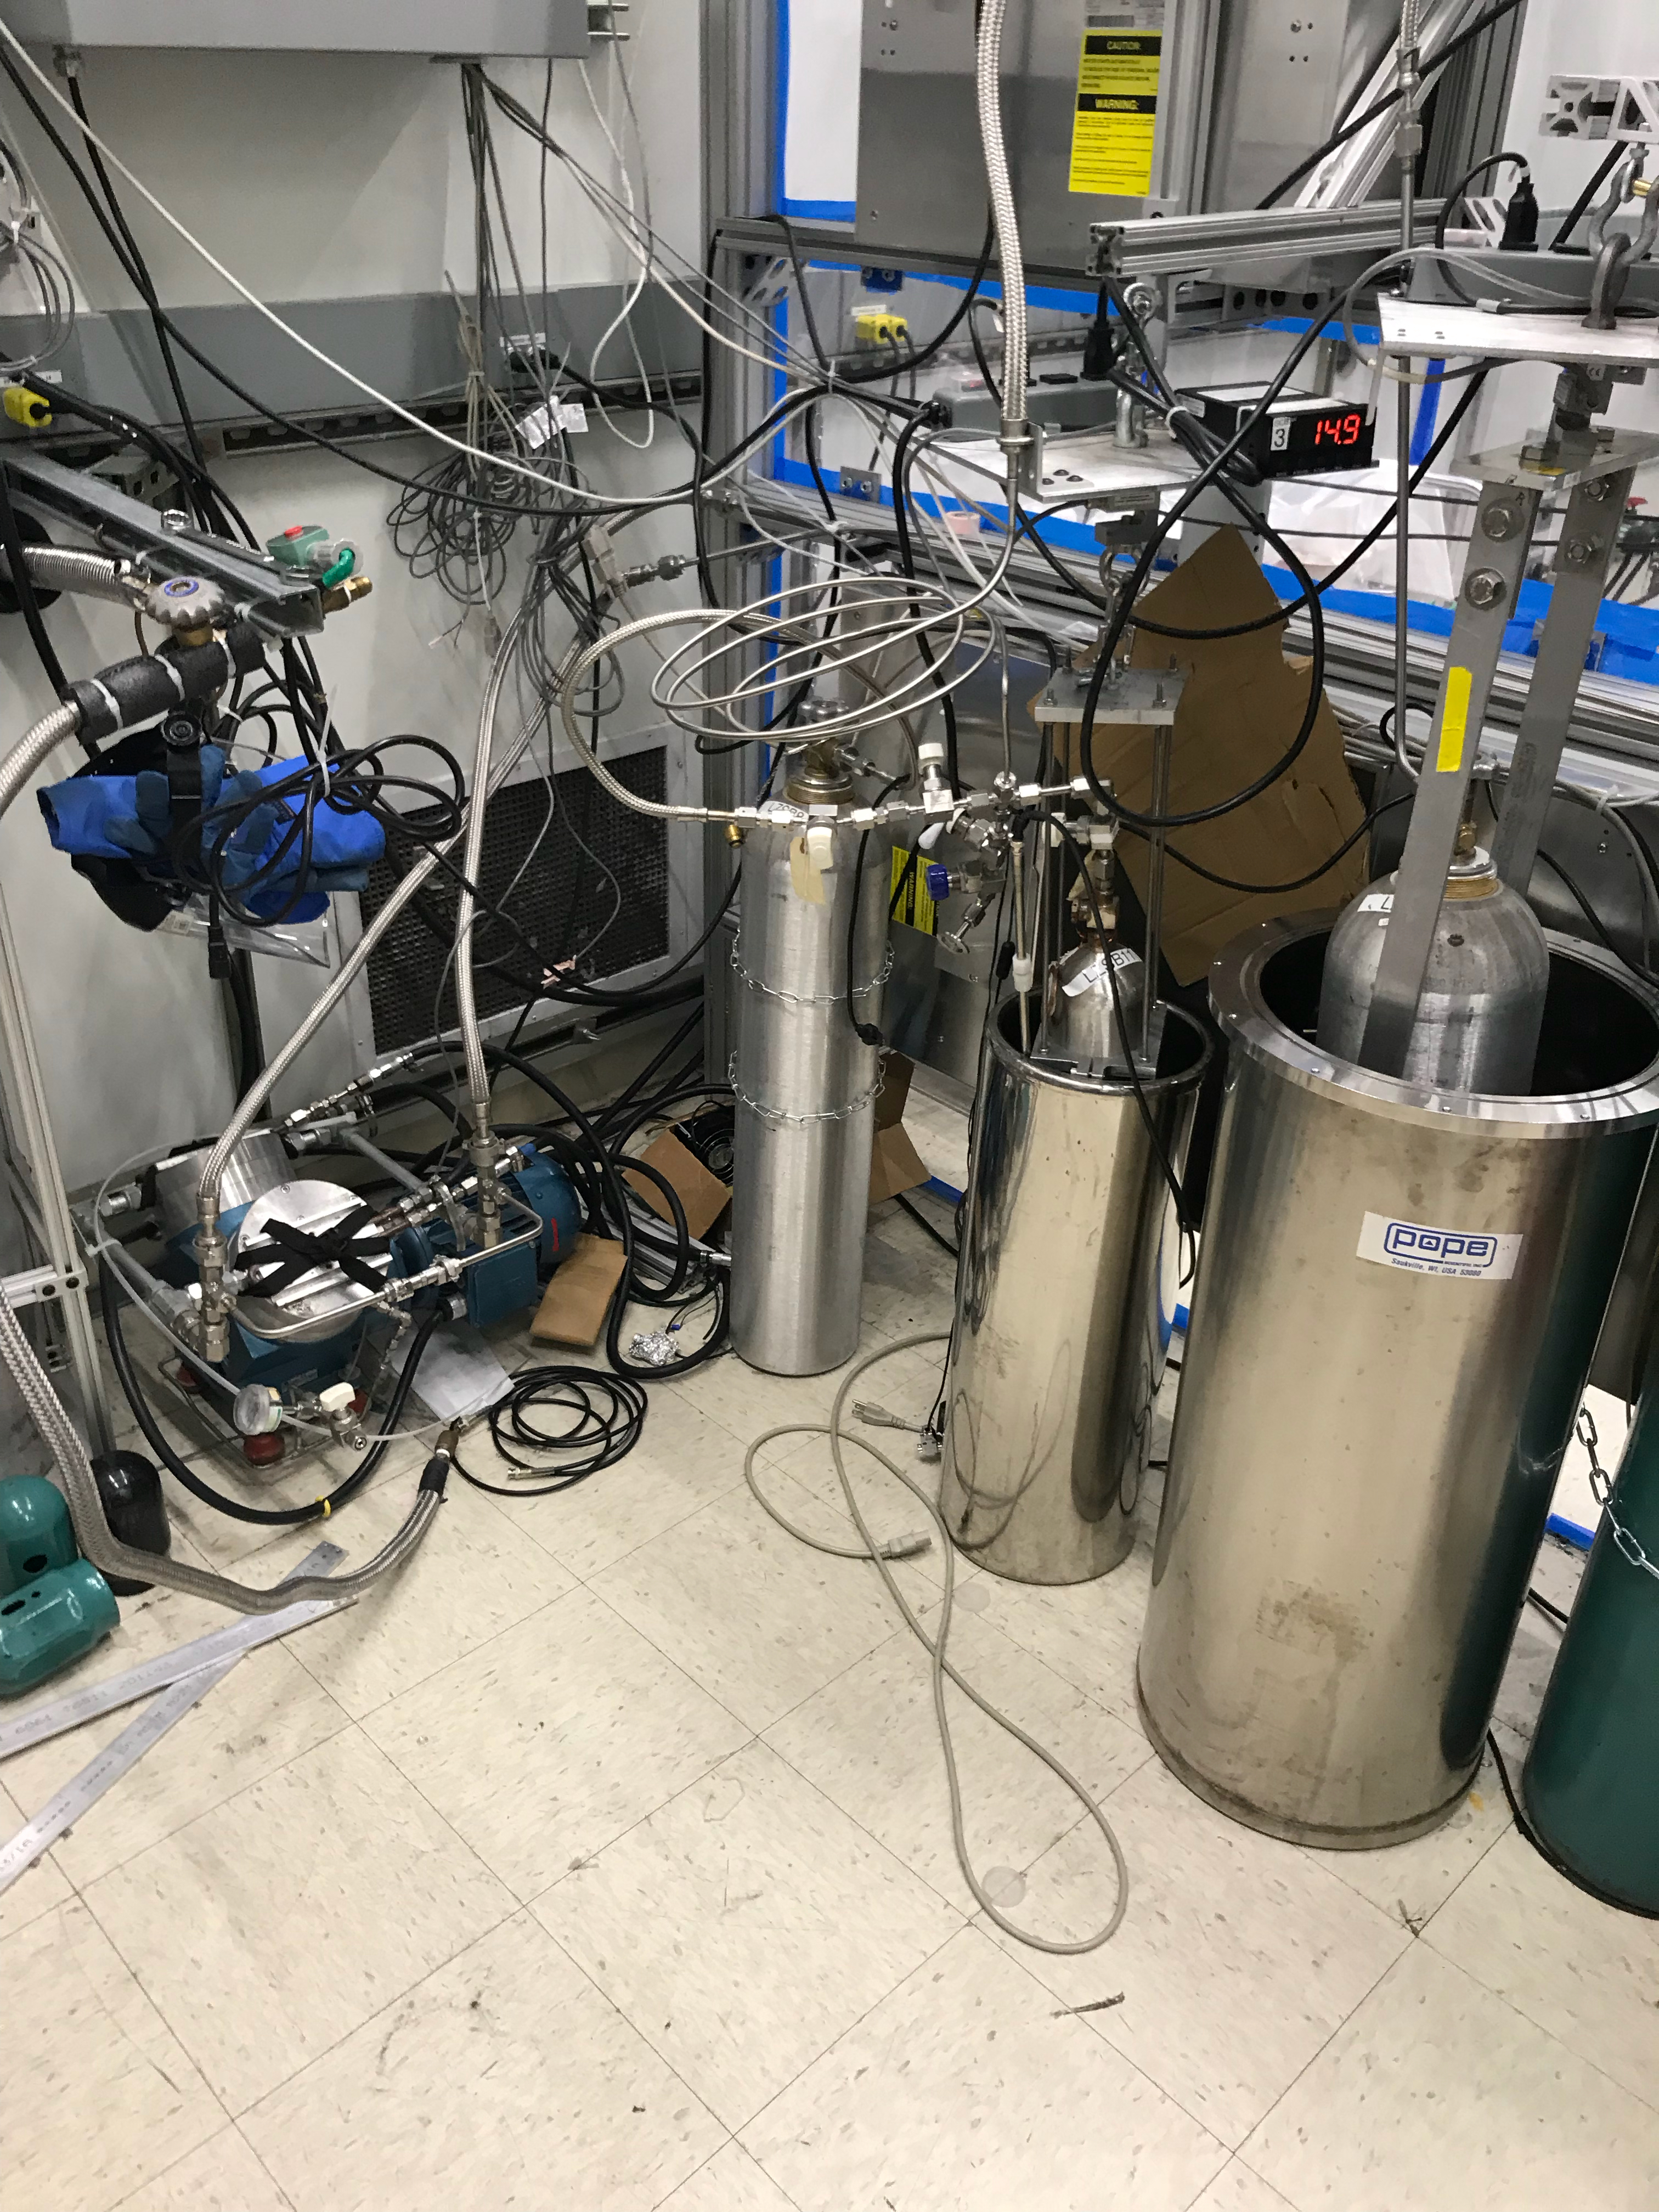
\includegraphics[width=\figurewidth,clip,trim={0 0 0 0},angle=0,origin=c]{Figures/GasTest/PhysicalLayout/GTBottles.jpg}
 \caption{}
 \label{fig:chambergeneral:bottles}
\end{subfigure}
\caption[\gtest\ apparatus physical layout]{\gtest\ apparatus physical layout: (a) the \gtest\ detector: detector vessel (middle),  electronic and gas gauge breakouts (top), Genie lift for detector assembly and disassembly (left), and vacuum pumping and leak check system (right), (b)  ELD inside the detector vessel, (c) gas circulation panel, (d) circulation pump (left), and storage bottles (right). }
\label{fig:chambergeneral}
\end{figure}

\paragraph{PMT} %f
Two PMTs are used to measure the primary scintillation and EL photons from events happens in the detector. Both PMTs are model R11410-20 PMTs manufactured by Hamamatsu Photonics, as described in Ref.~\cite{HamamatsuPhotonics2006}. The PMTs are named after their physical location in the detector as top PMT and bottom(bot) PMT. The spectral response of the PMTs tested in Hamamatsu company is summarized in Table.~\ref{tab:PMTparameterHamamatsu}.

\begin{center} 
\centering
 \begin{table}
    	\centering
\begin{tabular}[!tb]{ | m{16em} ||m{9em} | m{9em}| } 
 \hline
 &Top(top) PMT&Bottom(bot) PMT\\\hline\hline
 Serial Number & KB1163 & KB1170 \\\hline
 Cathode Luminous Sens. [\si{\uA\per\lumen}] & 149.0 & 148.0 \\\hline
 Anode Luminous Sens. [\si{\A\per\lumen}] & 657.0 & 1010.0 \\\hline
 Anode Dark Current [\si{\nA}] & 1.00 & 4.60 \\\hline
 Cathode Blue Sens. Index  & 12.60 & 12.30 \\\hline
 Q.E. [\si{\percent}] & &  \\\hline
 \quad \quad \SI{165}{\nm} & 22.1 & 21.2 \\\hline
 \quad \quad \SI{170}{\nm} & 33.3 & 32.6 \\\hline
 \quad \quad \SI{175}{\nm} & 36.3 & 36.0 \\\hline
 \quad \quad \SI{182}{\nm} & 37.1 & 37.0 \\\hline
 \quad \quad \SI{188}{\nm} & 36.1 & 36.2 \\\hline
 \quad \quad \SI{194}{\nm} & 33.9 & 34.1 \\\hline
 \quad \quad \SI{200}{\nm}& 32.6 & 32.9 \\\hline	
\end{tabular}
 \caption[Spectral response of PMTs tested by Hamamatsu Photonics]{Spectral response of PMTs tested by Hamamatsu Photonics.}
 \label{tab:PMTparameterHamamatsu}  
 \end{table}
\end{center} 

\section{Data Acquisition} %f1
A data acquisition(DAQ) system is used for recording PMT pulses for this experiment. It is designed and made in \slac . It was previous used and tested in \phaseone . It is customized to maximize the probability for capture single photon electron (\sphe ) pulses from the PMTs. This also enable the DAQ system to record photons from \eep . The DAQ system contains three parts: (1) amplification and digitization, (2) trigger, and (3) transfer and storage. The DAQ works continuously, except for interrupted by data transfer. This is called dead time of DAQ. %This set the limit of speed for DAQ.

\paragraph{Amplification and digitization} %f1
%purpose
The amplification and digitization system amplifies and digitizes the PMT pulse signals. It sets the precision of  \sphe\ measurement and signal to noise ratio. The amplification and digitization of the PMT signals are done by two separate custom made board. The amplification board amplifies the signal so that it improves signal to noise ratio. This eases background signal selections. There are two amplifier gains implemented: (1) low gain: $\times$ 12, and (2) high gain: $\times$ 100. For electron emission tests, the low gain setting is used to get enough signal to noise ratio. 
An optical fiber connecting these two boards transfers the amplified PMT signals to the digitizer board. The digitizer board is capable of doing a \SI{16}{\bit} digitization of pulse amplitude signals in a dynamic range of \SI{2.5}{\V}. The range of digitizing voltage is roughly \SIrange{-1.26}{1.24}{\V}. Digitized data are written to a buffer memory in the digitizer board. %This writing happens continuously, except for interrupted by data transfer. This is called dead time of DAQ, and will be explained below. 
The digitizer reverses polarity of signals. Fig.~\ref{fig:DAQPhysicalLayout} shows DAQ system physical layout.

\begin{figure}[!tb]
 \centering
 \begin{subfigure}[t]{\halfwidth}
    	    	\centering
   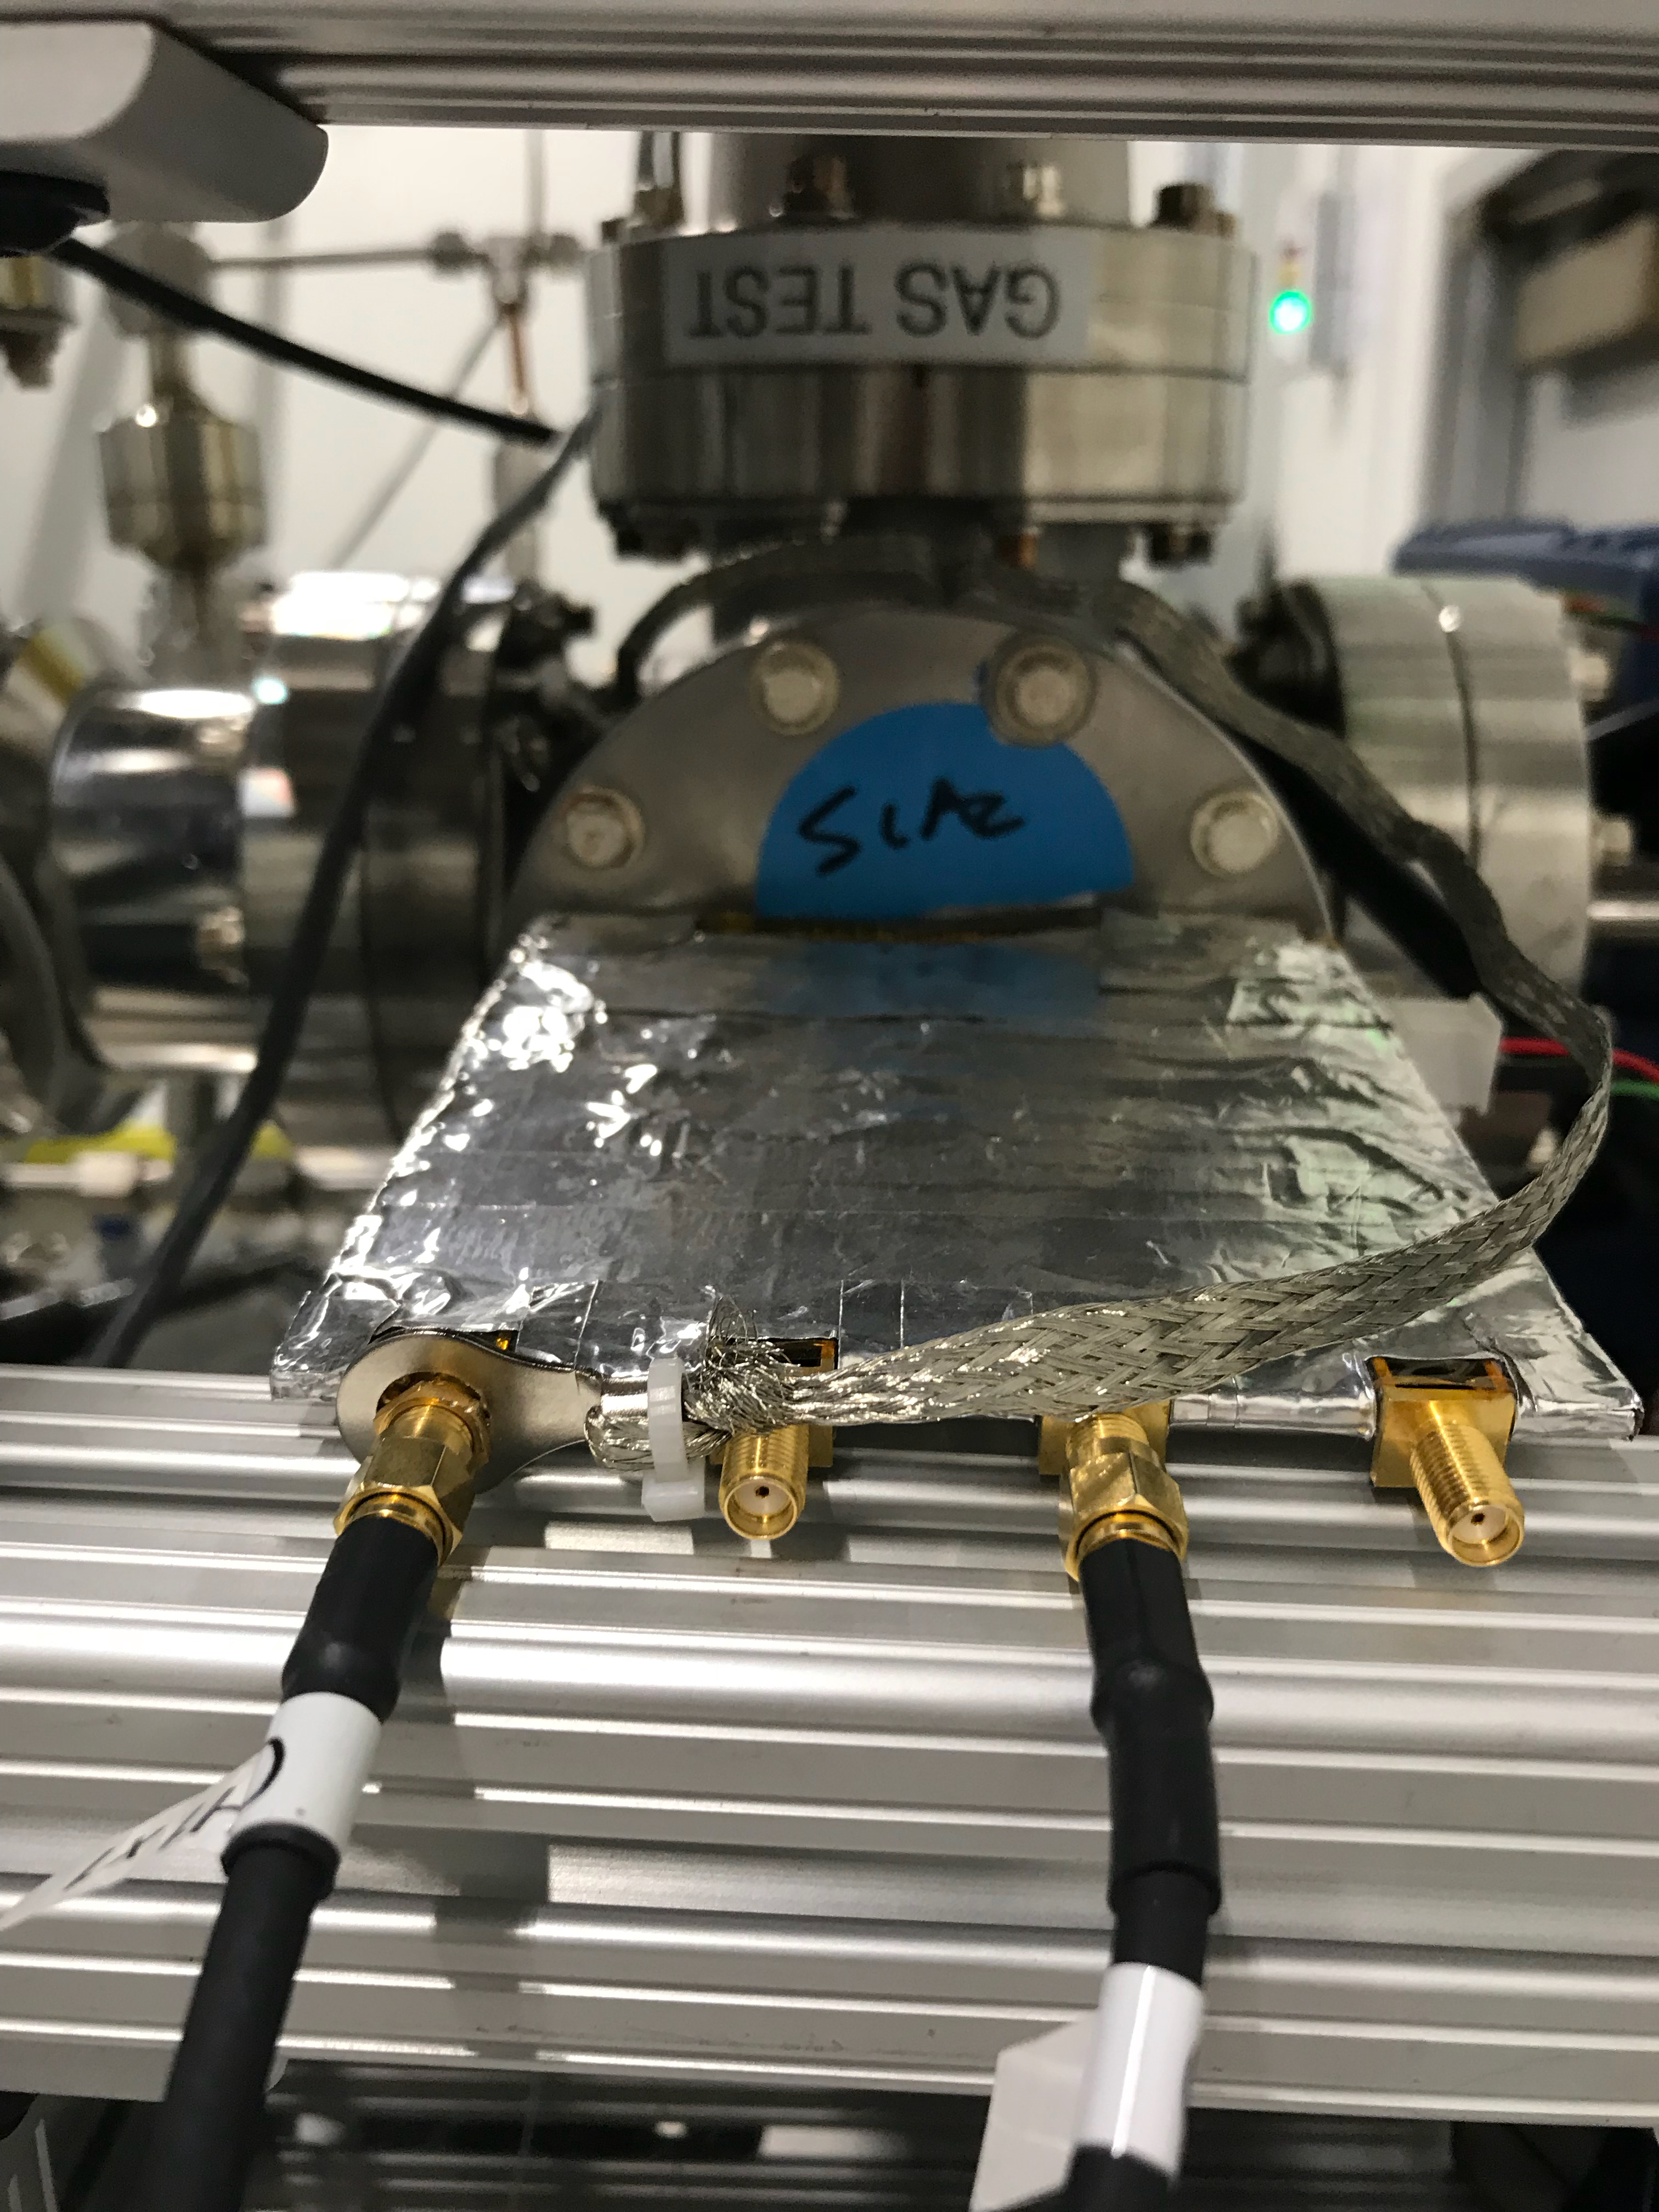
\includegraphics[height=15em]{Figures/GasTest/PhysicalLayout/PreAmp.jpg}
   \caption{}
   \label{fig:amplifier}
 \end{subfigure}
 \begin{subfigure}[t]{\halfwidth}
    	    	\centering
   \includegraphics[height=15em]{Figures/GasTest/PhysicalLayout/DigitizerInBox.jpg}
   \caption{}
   \label{fig:digitizer}
 \end{subfigure}
 \caption[\gtest\ data acquisition system physical layout]{\gtest\ data acquisition system physical layout: (a) amplifier board. (b) digitizer board.}
 \label{fig:DAQPhysicalLayout}
\end{figure}

\paragraph{Trigger} %f1 
The trigger system for DAQ makes decisions for data recording. Customized parameters in the DAQ trigger system are set in a XML file. These parameters are called XML parameters. The pulse trigger and recording is done in a pending mode which is  different from normal DAQ system. The continuous digitized pulse amplitude data are compared to the pre threshold value until finding a threshold crossing. This is the trigger time. Pulse recording will also including a preceding segment of samples, which is called pre delay. Digitized data are then compared to the post threshold value until finding a threshold crossing. Pulse recording will also including a following segment of samples, which is called post delay. During the post delay era, the digitized data are compared to the pre threshold again. If no threshold crossing is found, the pulse recording will end when the post delay era end. Otherwise, the DAQ will keep recording until after a post threshold crossing, no other pre threshold crossing can be found in the next post delay era. The pre threshold values are chosen so that the \sphe\ trigger efficiencies of both PMTs are larger than \SI{95}{\percent}. The trigger efficiencies are estimated by fitting \sphe\ amplitude distributions to Gaussian distribution curves. Results of these evaluations show that at normal PMT operation voltage(\SI{1.5}{\kV}) the top PMT and the bottom PMT have good trigger efficiencies of \SI{99.6}{\percent} and \SI{>99.9}{\percent}. 

The default settings for the DAQ XML parameters are summarized in Table.~\ref{tab:DAQparameters}.

\begin{center} 
  	\centering
  	\begin{table}
  	\centering
 \begin{tabular}[!h]{ | m{7em} ||m{7em} | m{5em}| m{15em}| } 
   \hline
   name & XML parameter name & value & explanation \\\hline\hline 
   post delay & 'PostDelay' &  \SI{500}{\sample} &counts of samples to keep after crossing post trigger threshold ('PostThreshold'). \\\hline
   pre delay & 'PreDelay' &  \SI{30}{\sample}& counts of samples to keep before crossing pre trigger threshold ('PreThreshold'). \\\hline
   post threshold & 'PostThreshold' & 0x7D80 or as needed &  crossing this threshold value determines the stop time of pulse recording.\\\hline
   pre threshold & 'PreThreshold' & 0x7D61 or as needed & crossing this threshold value determines the start time of pulse recording.\\\hline
 \end{tabular}
 \begin{flushright}
    	the sample size is \SI{4}{\ns}
 \end{flushright}
   \caption[Data Acquisition system parameters]{DAQ system parameters}
   \label{tab:DAQparameters}
\end{table}
\end{center}


\paragraph{Transfer and storage} %f1
The transfer and storage system transfers and storages data. The buffer memory data pass the selection of trigger algorithm are transferred through an optical fiber and written to the main computer. Data transfer speed is \SI{250}{\mega\byte\per\second}. For an average pulse duration of \SI{2}{\us} (\SI{500}{\sample}), the DAQ allows for approximately 30 thousand pulses to be recorded per second. Data are saved in binary format in the main computer.

\paragraph{Dead time} %f1
Dead time of DAQ is the segment of time that DAQ stops working after the end of each recording. Dead time brings challenges on measuring electron emission rates. 

The reason for dead time is because buffer writing and data transfer in the DAQ system cannot happen at the same time. 

Dead time in each PMT channel is independent from each other. Duration of dead time shows a dependence on the preceding pulse duration and pulse size. However, the quantitative relationship is unclear. 

Dead time is studied with finding the pulse that have large quantities of photons in one PMT and no record in the other PMT at the same time. These are potential dead time issue pulses. Causes of these issue pulses can also be misbehavior of one PMT or a large quantity of photon production inside one PMT. The time difference between the potential issue pulse in one PMT and the first preceding pulse in the other PMT is the potential duration of dead time. 
More than \num{400} dead time issue pulses are studied. For a pulse with a duration of \SI{2}{\us}, duration of dead time is in range \SIrange{0.3}{15}{\us}. Durations of dead time are observed in range up to \SI{80}{\us}.

Thus, a fraction of events that have quiet preceding are used to study the absolute rate of signals of interest. These resolves the dead time issue. DAQ trigger of the selected quiet preceding pulses are equivalent to DAQ trigger without the dead time issue. Details of how quiet preceding selection is done are discussed below in Section.~\ref{sec:uncor}.

\section{Operation} %f1

\todo{think about where to put run selection section. I want to take about , what is sparking test, what is normal operation before electron emission tests. This is the reason this section is here. however, put it just in front of cut might also be good.}

The run selections are to make sure that we have stabilized run conditions to analysis electron emission process from grids we are studying. %It makes it possible for us to compare results between different runs. 

\paragraph{Operation conditions} %f1
The normal run of \gtest\ electron emission test is operated with (1) the detector filled with xenon gas, (2) two PMTs stably running, and (3) two grids bias to proper voltages. 

The typical operation xenon gas density for electron emission tests is \SI{0.137}{\mole\per\liter} (or equivalent to the xenon gas density at \SI{177}{\kelvin} on xenon liquid-vapor saturation curve). This choice is made to have the gas density closest to \lze\ operation gas density. It also minimizes the probability of discharges between two grid electrodes. These discharges may cause potential damages to grids, and also prevent stable run. 

The gas operation condition at density \SI{0.137}{\mole\per\liter} allows us having sensitivities measuring electron emission from \opdv\ in range \SIrange{8}{16}{\kV}. For a plain woven grid with wire pitch \SI{5}{mm} and wire diameter \SI{75}{\um}, this correspond to an average \wsef\ in range \SIrange{65}{110}{\kV\per\cm}. However, the photon yield per electron emission is smaller for a lower \opdv . This prevents us to have enough sensitivities for electron emission for a lower operation voltage and \wsef . So electron emission rate for a lower \wsef\ is measured at a lower gas density to get enough photon yield. 

Two PMTs normally operate at \SI{1.5}{\kV}. This guarantees both PMTs having enough gain and signal to noise ratio. Before safely turning on the PMTs to measure the light emission from the grids, a series of sparking tests are done to figure out the high voltage behavior and high voltage weak points in the system. Improvements are done to improve the maximum \opvtvb . These improvements include cleaning the surface of discharging spots, increasing the smoothness and rounding radius on the corner of metal surfaces, and increasing the discharge distance between electrodes and the ground. Touching grid wires are avoided during these improvements. The maximum \opvtvb\ that these grids can hold are measured with different gas and different pressures. Dark current of both PMTs in stable running condition are approximately \SIrange{500}{1000}{\Hz}. Run with any PMT dark current rate above \SI{2500}{\Hz} are excluded. 

The high voltage power supply is capable to bias both grids separately in range \SIrange{-8}{8}{\kV}. The current between the power supply and the grid is monitored to guarantee stable operation of grid bias voltage. An unstable grid biasing usually shows as a spike in the monitored current, and a spike on PMT recording rates. Segments of time with this monitored current unstable are excluded.  

\paragraph{Operation data talking} %f1
The most common operation voltage pairs we choose for electron emission measurement at xenon gas density \SI{0.137}{\mole\per\liter} are $V_{T}=-V_{B} $ at \SIlist{\pm 4; \pm 4.5; \pm 5; \pm 5.5;\pm 6; \pm 6.5;\pm 7; \pm 7.5;\pm 8}{\kV}. This allows us to measure electron emission rate vs \opdv\ curves for most grids we study. Measurements in other conditions are also performed to understand the detector better. However, their results usually are not included for the electron emission studies.

The typical duration of data taking is three minutes. An increasing trend of light production is seen during the operations when data taking is longer than three minutes. This is probably from the increment of EL light production from the more ionized chamber environment and increment of fluorescence light emission from PTFE reflector cones in the detector. Usually, after each \SI{3}{\min} dataset, high voltage power for both grids are set back to \SI{0}{\kV} and rest for at least \SI{30}{\s} before the next measurement. 

Datasets with the lower value of two grid bias voltages higher than \SI{-2.5}{\kV} are explicitly excluded for electron emission measurements. The reason is because this configuration allows electrons created by external particle in the cone region drifting to the EL region. These electrons will produce EL light in the EL region. This could introduce a significant background for electron emission rate study. The process is illustrated in Fig.~\ref{fig:BelowCathodeIllustration}.

\begin{figure}[!p]
 \centering
 \begin{subfigure}[b]{\halfwidth}
 			\centering
   \includegraphics[width=\figurewidth,clip,trim={0 0 0 0},angle=0,origin=c]{Figures/GasTest/WeiDrawEvent/GoodConfig.jpg}
   \caption{}
   \label{fig:BelowCathodeIllustration:GoodConfig}
 \end{subfigure}
 \begin{subfigure}[b]{\halfwidth}
 			\centering
   \includegraphics[width=\figurewidth,clip,trim={0 0 0 0}]{Figures/GasTest/WeiDrawEvent/BadConfig.jpg}
   \caption{}
   \label{fig:BelowCathodeIllustration:BadConfig}
 \end{subfigure}
 \caption[\gtest\ good and bad voltage configurations]{(a) good configuration ($V_{C} < V_{PMT}$) : drift field is pointing from PMT to the grids. Electrons created in the cone region will drift to PMT. This process do not create many photons. (b) bad configuration  ($V_{C} > V_{PMT}$) : drift field are pointing from grids to the PMT. Electrons created in the cone region will drift to EL region. This process create lots of EL photons and could look like an \eep .}
 \label{fig:BelowCathodeIllustration}
\end{figure}

\section{Data processing} %f1
Data processing is to reduce the dimensions of data and to save the useful informations of data. This reduces size of analysis works. The useful informations of a pulse are characterized by Reduce Quantities of a pulse (RQs).

The data processing framework include three parts: (1) single pulse processing, (2) coincidence event building and coincidence pulse processing, and (3) random segment sampling of the dataset.

This section explains the main part of data processing framework. It does not mean to explain all the RQs that have been computed. A full documentation of the RQs used in \gtest\ analysis is summarized in Appendix.~\ref{chapter:gastestRQ}.

\paragraph{Single pulse processing} A single pulse is defined to be the individual pulse recorded by DAQ system in only one PMT channel. Two steps are done for this processing: (1) waveform reconstruction, and (2) pulse shape characterization. 

The waveform is reconstructed with the following method. The average DC bias of the pulse of the first 10 samples was calculated as the baseline of the pulse (RQ name: 'baselines'). These samples are \SI{80}{\ns} ahead the trigger time of the pulse. In principle, baseline voltages are not effected by the following pulses. Thus, they reflects DAQ quiet bias voltages. There are some smaller fluctuation of baseline voltages for both PMTs. The amplitude of fluctuation \SI{\sim 0.36}{\mV} is very small comparing to \sphe\ pulse amplitude, which is \SIrange{15}{35}{\mV}. After baseline finding, the baseline value was subtracted from the digitized data to get the waveform for the pulse. The waveform is then scaled back from ADC counts to \si{\mV} to get the reconstructed waveforms. Along this process, RQs for the voltage of the trigger sample (RQ name: 'trigvals'), the voltage of the first sample (RQ name: 'firstvals') are also calculated.

From the reconstructed waveform, the maximum positive amplitudes(RQ name: 'waveamplitudes') and the pulse area (RQ name: 'waveareas'), which is the time integral of the pulse amplitude are calculated. However, because of the long post delay duration (\SI{2}{\us}, \SI{500}{\sample}) from the DAQ pulse recording, baseline fluctuation during the post delay era is included in the total time integral of the pulse area. This biases our understanding of pulse area. Thus, another revised pulse area RQ (RQ name: 'waveareas\_trim\_end') is calculated from integrating the waveform with removing the last \SI{1.8}{\us}, \SI{450}{\sample} from the end of the waveform. This revised pulse area RQ is used in main analysis instead for PMT pulse area calibrations. 
%We also calculated the integrated duration of the pulse amplitude larger than the noise level (RQ name: 'pos\_len\_above\_threshold\_trim\_end'). This is used for \sphe\ pulse judgment.     

Series of pulse shaping parameters are also calculated. Time weighted integral of waveform (RQ name: 'wtimeN') is used to study the skew and kurtosis of the pulse. Also, time difference between the start time of the pulse and time that the integrated area of the pulse reaches several different portions of the total pulse area are calculated. They are the characteristic time differences of the pulse (RQ name: aft\_tXX). They are very useful for understanding the pulse shape, pulse duration, and pulse center of mass. These help pulse selection and classification discussed in the following sections. 

\paragraph{Coincidence event building and coincidence pulse processing}  \label{par:coinbuild}
The DAQ system records pulses in each PMT channel independently. A true \eep\ usually can produce enough quantity of photons to be recorded by both PMTs. So RQs of coincidence pulses between two PMTs contain more useful informations for \eep s. 

The coincidence event building requires triggers in both PMTs. It is done in a pending searching. From a single pulse, two segments of time were subtracted from the beginning and end of the pulse to reduce the influence from the baseline fluctuation in the PMT. The default values for post pulse subtraction and pre pulse subtraction is \SI{1800}{\ns} (\SI{450}{\sample}) and \SI{0}{\ns} (\SI{0}{\sample}). This beginning and ending time of the remained part of the pulse is called the start ($t_{start}$) and the stop time ($t_{stop}$) of the pulse. Then, a pulse searching is performed between a certain segment of time before the start of the pulse and the same amount of time after the stop time of the pulse. The value of additional segments of time looking for coincidence pulses is coincidence window width (CWW, RQ name 'window\_width'). If no other pulse is found in this time region, no coincidence pulse is found for this particular single pulse. If another pulse is found in this time region. Then, the start and the stop time of the coincidence pulse are extended to cover the start and the stop time of the new found pulse. The new found is added to form a group with the previous single pulse. This group is called coincidence pulse. Another round of coincidence searching is performed again with the same algorithm with the addition of the new pulse. Searching continues until no other pulse matches this criteria can be found. That is no other recorded single pulse has its start time and stop time in the searching window of the group of coincidence pulse .

The value of CWW for this analysis is \SI{1.7}{\us}, if not otherwise specified. The coincidence pulse is defined as the addition of normalized pulses in each channel. The normalization is performed by dividing the pulse amplitude by the \sphe\ pulse area in that channel. A similar pulse characterization is performed for the coincidence pulses as in single pulse processing.    

Some commonly used coincidence pulse RQs are listed below. They are
\begin{itemize}
\item coincidence pulse area: RQ name 'coin\_pulse\_areas\_norm', pulse area of coincidence pulse, measured in \si{\phe}.
\item $t_{\text{XX}}$: RQ name 'coin\_pulse\_areas\_tXX', time difference between the start of the coincidence pulse and integrated pulse area reach XX \% of the total coincidence pulse area, measured in \si{ns}. XX = 01, 05, 10, 15, 25, 50, 75, 85, 90, 95, 99.
\item \tzeronine : $t_{99}-t_{01}$, also is noted as \pud .
\item \ttenninety : $t_{90}-t_{10}$, also is noted as \rpd .
\item \ttwoseven : $t_{75}-t_{25}$
\item section 1 area: RQ name 'coin\_pulse\_areas\_section1', coincidence pulse area in the first \SI{300}{\ns} from the start time of the coincidence pulse, measured in \si{\phe}.
\item section 2 area: RQ name 'coin\_pulse\_areas\_section2', coincidence pulse area in the first \SI{800}{\ns} from the start time of the coincidence pulse, measured in \si{\phe}.
\item TBA: top bottom asymmetry, TBA $\equiv$ (T-B)/(T+B),  where T is the pulse area in the top PMT and B is the pulse area in the bottom PMT. 
\end{itemize}

\paragraph{Random segment sampling}
The event rates are checked by looking at pulses around a random sample of times during the operation. In each dataset, 10,000 random times are chosen. From each random time, total pulse area in the preceding and the following \SIlist{10;20;50;100}{\us} windows are calculated. These values of random sampling represent the average photon density in the detector in this dataset. They are compared to other segments of time of interest to study correlation light productions.  
%Comparing these statistics to same quantity from period of time before and after certain type of event allows us finding the correlation of events in the detector.     

\section{PMT Calibration}
\label{sec:pmt cal} 
PMT calibrations are performed for understanding the trigger efficiency, pulse amplitude, and pulse area of a \sphe\ for each PMT. \sphe\ trigger efficiencies of a PMT determines the event recording efficiencies. \sphe\ pulse amplitude of a PMT determines the capability of DAQ to record the full height of a sized pulse. \sphe\ pulse area of a PMT is the fraction denominator we use to calculate the counts of photon electrons in each pulse. Counts of photoelectrons in each pulse are roughly estimated by, 

\begin{align}
  	\text{\# photoelectrons in a pulse [\si{phe}]} \sim \frac{\text{total pulse area}}{\text{single photon electron pulse area}}
\end{align}     

Datasets that are used in the calibration are taken at vacuum and \opvtvb\ at \SI{0}{\kV}. The detector in this condition will have the minimum influence from events from internal and external sources. Thus, a cleaner population of \sphe\ can be selected. 
  
% 2017 Dec 8th 14:02, with detector standard xenon gas density and operation voltage (dV) at \SI{12}{\kV}. 
  
\paragraph{PMT trigger efficiency}
PMT trigger efficiency is estimated by comparing its trigger voltage to its \sphe\ amplitude distribution. A simple Gaussian distribution is used to represent the distribution of \sphe\ amplitude. A fit range in amplitude of is chosen to avoid the influence from noise and overlapping of multiple photo electrons. The fit range is \SIrange{12}{28}{\mV} for the top PMT, and \SIrange{22}{38}{\mV} for the bottom PMT. The range choices are \SI{\sim \pm 8}{\mV} from the center peak values of the \sphe\ pulse amplitude. The trigger voltage of each PMT is compared to the survival function (complementary cumulative distribution function) of the fitted Gaussian distribution to get the trigger efficiency. Results of curve fittings are shown in Fig.~\ref{fig:PMTTriggerEff}. The figures show a close to unity trigger efficiency of both PMTs.
  
\begin{figure}[!h]
	\centering
	\begin{subfigure}[b]{\halfwidth}
		\centering
		\includegraphics[width=\textwidth,clip,trim={0 0 0 0},angle=0,origin=c]{Figures/GasTest/DatasetQuality/topPMTTriggerEfficiency65831.jpg}
		\caption{}
		\label{fig:PMTTriggerEff top}
	\end{subfigure}
	\begin{subfigure}[b]{\halfwidth}
		\centering
		\includegraphics[width=\textwidth,clip,trim={0 0 0 0}]{Figures/GasTest/DatasetQuality/botPMTTriggerEfficiency65831.jpg}
		\caption{}
		\label{fig:PMTTriggerEff bottom}
	\end{subfigure}
	\caption[PMT pulse amplitude distribution]{PMT pulse amplitude distribution: (a) top PMT (b) bottom PMT. Data were taken at \ddtt{2018}{03}{12}{11}{41}.}
	\label{fig:PMTTriggerEff}
\end{figure}

\paragraph{PMT \sphe\ pulse area}
 PMT \sphe\ pulse area is calibrated with fitting the pulse amplitude and integrated area to a two dimensional Gaussian distribution. The used fitting function is, 
 \begin{align}
 	A \exp \bigg( -\Big(\frac{1}{2 \sigma_x^2} \big( (x-\mu_{x})\cos \theta - (y-\mu_y)\sin \theta \big) ^2 + \frac{1}{2 \sigma_y^2} \big( (x-\mu_{x})\sin \theta + (y-\mu_y)\cos \theta \big) ^2  \Big) \bigg)
 \end{align} 
where A, $\mu_{x}$, $\sigma_{x}$, $\mu_{y}$, $\sigma_{y}$, and $\theta$ are the fitting parameters.  

The mean values for pulse area and pulse amplitude are $\mu_{x}$ and $\mu_{y}$. The standard deviation values for pulse area and pulse amplitude are $\sigma_{x} \cos \theta - \sigma_{y} \sin \theta$ and $\sigma_{x} \sin \theta + \sigma_{y} \cos \theta$. Results of these fits are shown in Fig.~\ref{fig:PMTAmpArea}. Results from PMT calibrations are summarized in Table.~\ref{tab:PMTparameters}. Fitting values of different dataset show an agreement within \SI{1}{\percent} on the mean PMT single photon electron pulse area and pulse amplitude. 

The values of \sphe\ pulse amplitudes are approximately \SI{20}{\mV} for the top PMT and \SI{30}{\mV}. Thus, a naive estimation shows the DAQ system allows approximately 60 \sphe s to be simultaneously recorded by the top PMT without distortion of pulse shape. The number of this is 40 for the bottom PMT. This dynamic range is large enough for record \eep\ without pulse shape distortion in most situations. 

Degrading of PMTs is noticed during the run. Technical details for this is discussed in Ref.~\cite{HamamatsuPhotonics2006}. However, since this effect is not significant during the tests. For consistency of studying, the same value for PMT \sphe\ pulse area is used through all the studies. 

There are two revisions of these values of SPHE pulse area. In revision 1 (Rev1), the values used are \SI{426}{\mV\ns} for the top PMT and \SI{638}{\mV\ns} for the bottom PMT. This is from analyzing pulse area on datasets taken with the detector filled with xenon gas and \opvtvb\ higher than \SI{0}{\kV}. These datasets contains more multiple photon electron pulses and biased the estimation. In revision 2 (Rev2), data taken at vacuum condition with \opvtvb\ at \SI{0}{\kV} are used. The values used are \SI{413}{\mV\ns} for the top PMT and \SI{610}{\mV\ns} for the bottom PMT. Rev2 gives a better estimation on \sphe\ pulse area. \sphe\ pulse area is noted as PHE below.

\begin{figure}[!h]
	\centering
	\begin{subfigure}[b]{\halfwidth}
		\centering
		\includegraphics[width=\textwidth,clip,trim={0 0 0 0},angle=0,origin=c]{Figures/GasTest/DatasetQuality/topPMTArea65831.jpg}
		\caption{}
		\label{fig:PMTAmpArea top}
	\end{subfigure}
	\begin{subfigure}[b]{\halfwidth}
		\centering
		\includegraphics[width=\textwidth,clip,trim={0 0 0 0}]{Figures/GasTest/DatasetQuality/botPMTArea65831.jpg}
		\caption{}
		\label{fig:PMTAmpArea bottom}
	\end{subfigure}
	\caption[PMT \sphe\ pulse amplitude vs pulse area distribution]{PMT \sphe\ pulse amplitude vs pulse area distribution: (a) top PMT (b) bottom PMT. Black dot, and dashed line are mean, \SI{68}{\percent}, and \SI{95}{\percent} contours of the Gaussian fits. Data were taken at \ddtt{2018}{03}{12}{11}{41}.}
	\label{fig:PMTAmpArea}
\end{figure}
\todo{think about whether to delete the first vacuum data in the table.}
\begin{center} 
\centering
	\begin{table}[!h]
	\centering
		\begin{tabular}[!h]{ | m{9em} ||m{5em} |m{5em} | m{5em} | m{5em}| m{5em}|} 
		\hline
		time & PMT name & trigger \mbox{voltage}  & trigger \mbox{efficiency} & pulse \mbox{amplitude}  & pulse \mbox{area} \\
   & & [\si{\mV}] & & [\si{\mV}] & [\si{\mV\ns}]
		\\\hline\hline

        \ddtt{2017}{08}{26}{11}{53}* & top & 3.679 & 0.997 & \num{18.4 \pm 4.1} & \num{395 \pm 118}   \\\cline{2-6}& bottom & 2.629& 1.000 & \num{28.6 \pm 6.0} & \num{599 \pm 155}\\\hline %proc33001

        \ddtt{2018}{02}{03}{13}{21} & top & 3.762 & 0.997 & \num{19.4 \pm 3.3} & \num{413 \pm 132}   \\\cline{2-6}& bottom & 3.103& 1.000 & \num{27.9 \pm 4.6} & \num{607 \pm 161}\\\hline %proc10201
		
		\ddtt{2018}{03}{12}{11}{41} & top & 3.853 & 0.996 & \num{19.3 \pm 3.5} & \num{411 \pm 130}   \\\cline{2-6}& bottom & 3.130& 1.000 & \num{29.2 \pm 5.1} & \num{607 \pm 161}\\\hline %proc65831

%		\ddtt{2018}{03}{16}{17}{49} & top & 3.788 & 0.996 & \num{19.4 \pm 3.4} & \num{413 \pm 128}   \\\cline{2-6}& bottom & 3.269& 1.000 & \num{29.4 \pm 5.3} & \num{614 \pm 164}\\\hline %proc65901
				
		\ddtt{2018}{05}{15}{12}{03} & top & 3.713 & 0.997 & \num{19.4 \pm 3.5} & \num{413 \pm 131}   \\\cline{2-6}& bottom & 3.091& 1.000 & \num{29.5 \pm 5.4} & \num{615 \pm 167}\\\hline %proc13001
%		\ddtt{2017}{12}{08}{14}{42} & top & 3.914 & 0.996 & \num{20.1 \pm 3.8} & \num{426 \pm 136}   \\\cline{2-6}& bottom & 3.245& 0.999 & \num{30.7 \pm 5.9} & \num{638 \pm 177}\\\hline
%		\ddtt{2018}{06}{06}{02}{35} & top & 3.932 & 0.996 & \num{19.9 \pm 3.7} & \num{423 \pm 133}   \\\cline{2-6}& bottom & 3.403& 1.000 & \num{30.5 \pm 5.8} & \num{633 \pm 173}\\\hline
	\end{tabular}
	
	\caption[PMT calibration]{PMT \sphe\ calibration. *: DAQ setting for trigger voltage, post delay, and number of sample trimmed at the end are different. The number of samples kept after post threshold are the same. }
 \label{tab:PMTparameters}
	\end{table}
\end{center}

\section{Light Collection}
\gtest\ studies event-based primary scintillation light and EL light. Light collection efficiency is important to understand the overall sensitivity of the detector.  

\begin{align}
\text{light collection efficiency} = \frac{\# photon created during an event}{\# photoelectrons seen by PMTs in an event}
\end{align}

Light collection efficiency includes geometric collection efficiency and PMT response. Geometric collection efficiency describes the efficiency of the photon propagation in gas media, photon reflection by the detector material surfaces, and photon absorption on PMT photocathode surfaces. PMT response describes the efficiency of how much photons hitting the photocathode turning into measurable current or voltage signals.

\paragraph{Geometric collection efficiency} Geometric collection efficiency is studies by photon propagation simulation software Light Guide, as described in Ref.~\cite{Shutt2018}. In the simulation software, a cylindrical symmetric simplified \gtest\ ELD geometry boundary is drawn to represent the real detector material surfaces that reflect and absorb photons. This simplified geometry includes the photocathode surface of PMTs, inner surface of the PTFE cones, and surfaces of the grid rings. Grid wire surfaces are represents by series of parallel wires with the same diameter and half the pitch distance as the real detector. The reason for using half the pitch distance is because the grid wires in the detector are two dimensional woven. Their quantities are twice larger than one dimensional parallel wires. The empty space inside the simplified ELD geometry is filled with transparent or translucent media. This software simulates photon propagation in transparent or translucent media using the physics quantity scattering and absorption of the media. 

To understand geometric collection efficiency at one specific spatial location, (r, z). num{10000} simulations of single photons are generated at the specific location. Each simulated photon takes steps to either transport through detector media or interact with detector surface materials. Each simulation ends when the simulated photon is absorb by either detector media or detector surface materials. Among all detector surfaces, the counts of photons reaching PMT photocathode surfaces are used to estimate geometric collection efficiency,  
\begin{align}
	\text{Geometric collection efficiency} = \frac{\# photons reaching PMT photocathode surfaces}{\# photons simulated}
\end{align}

\paragraph{PMT response} PMT response includes (1) PMT quantum efficiency (Q.E.)., (2) PMT electron collection efficiency ,and (3) PMT electron gain. 

PMT Q.E. is the ratio of output photoelectrons to incident photons. It is the efficiency of photoelectric effect including the probability of photoelectric effect creating multiple photoelectrons from a single photon (double photoelectrons effect).  
We use counts of photoelectrons detected (PHD) to describe the counts of photons detected without the influence of double photoelectrons effect, and counts PHE to describe the counts of photons detected with the influence of double photoelectrons effect. 
Statistical average one PHD is approximately \num{1.2} PHE. PHE is the unit that is used in this analysis. 
In this simulation, values of PMT Q.E. at \SI{175}{\nm} are used. They are \SI{36.3}{\percent} for the top PMT and \SI{36.0}{\percent} for the bottom PMT, see Table.~\ref{tab:PMTparameterHamamatsu}. 

PMT electron collection efficiency is the probability that these output photoelectrons land on the effective area of the first dynode. This makes the electrons go to the next dynode and being multiplied by the chains of dynodes. PMT electron collection efficiency depends on PMT mechanical design and the voltage difference between the PMT photocathode and the first dynode. The exact electron collection efficiency of the PMTs used in \gtest\ at their operation voltage are not measured. We estimate PMT electron collection efficiencies to be \SI{90}{\percent} based on measurement of other PMTs of the same model at a higher PMT operation voltage, as described in Ref.~{Lung2012
	%,Akerib2013b
}.

PMT electron gain describes the multiplication process of the electron in dynode stage. The voltage of the multiplication is the PMT signal we measured. The multiplication of electrons amplifies the useful signal and eases the signal noise selection. The mean value of the time integrated voltage is mean pulse area in PMT calibration. The coefficient of variation (CV, the ratio of the standard deviation to the mean value) for mean pulse area is \SI{\sim 30}{\percent}, as described in Section.~\ref{sec:pmt cal}. 

So, for understanding the spacial dependence of the light collection in the ELD, we start with \num{10000} every \SI{1}{\cm} in r and z dimension in the ELD, and record the geometric collection efficiency of each location. This number is then multiplied by PMT Q.E. and PMT electron collection efficiency to get the total light collection efficiency. Fig.~\ref{fig: light col old} shows results of these simulation. Geometric collection efficiency varies at different spacial locations in the detector and cause light collection efficiency also varies. Top bottom asymmetry (TBA), which is the ratio of top PMT collection collection efficiency to bottom PMT light collection efficiency also varies across the ELD. We

\begin{align}
	\text{TBA} = (1+\text{TBR})/(1-\text{TBR})
\end{align}

Locations that are in the top cone region get a larger than one TBR, and locations that are in the bottom cone get a  


Among all different classes of events, our primary pulse of interest is \eep . 


  \todo{A statistical fluctuation of \SI{30}{\percent} are added.}

\section{Cuts}
\todo{I think I should arrange the cuts by what I think is the origin of the cuts rather than category by pulse shape and uncorrelation. think about it more.}

This section discusses pulse selections, aka cuts, that are used in \gtest\ analysis. The purpose of this analysis is searching for \eep s from tested grid wires and correctly estimating the rate of this process. Pulse selections are done on different parameter spaces. For each pulse selection, possibility of removing signals of interest (in this case: \eep ) is evaluated. The primary principle of pulse selections is to get a clean population distribution of \eep\ to get a reliable estimation of its rate. Other than that, since \eep\ s are in most situation rare in the detector, pulse selections of these \eep s are done conservatively. That is to keep as many candidates for \eep s as possible. 

An \eep\ should: 
\begin{itemize}
\item be an uncorrelated pulse from previous pulses in time, and
\item have the correct pulse shape.
\end{itemize}

To make the pulse selections, a study of the \eep\ is done for understanding its pulse shape. Background events that originate from different source will be separately discussed. Their pulse shape and rate are studied. The cuts that removes these backgrounds are described. Finally, the efficiencies of these cut and their potential of removing good \eep\ candidates are estimated. Corrections for these efficiencies in this analysis are also described in the end.  

\subparagraph{Electron emission} A cartoon for the physical process and an example waveform of \eep\ are shown in Fig.~\ref{fig:eep}. An electron leaves the cathodic electrode from various types of emission processes. After the electron left the wire surface, the high electric field around the cathodic wire will quickly energize the electrons. The high energy electron ionizes and excites the atoms around it and create more electrons. In this region, more EL light is produced per second comparing to a lower electric field region. This is the cause of the "peak" at the beginning of the \eep . This process is called electron multiplication. Then, these electrons drift to the anodic electrode due to the operation voltage difference between the two grids. EL light is produced along this drift. This correspond to the majority of EL light seen in the \eep . There is a clear start and stop time for the \eep . Duration of the \eep\ is roughly the duration of this drift. After this, electrons get close to the anodic electrode. Since the electric field around the anodic wires are also high, electrons also go through a similar electron multiplication process. This process also creates more electrons and a higher density of EL light. This is the cause of the "peak" at the ending of \eep . The peak at the end of the pulse is lower than the peak at the beginning of the pulse. This is because of dispersion of the arrival times of electrons on anodic electrode. This dispersion is due to the different microscopic trajectory each electron takes to reach the anodic electrode. Different arrival times of the electrons cause the final increment of EL light productions from different electrons do not happen coincidently. This lowers the height of the peak at the ending of the \eep . Another reason for the different height of the peak is due to the electric field on the anodic wire is smaller than cathodic wire. It also results in a smaller production of EL light.

\begin{figure}[!p]
	\centering
	\begin{subfigure}[b]{\halfwidth}
		\centering
		\includegraphics[width=\figurewidth,clip,trim={0 0 0 0},angle=0,origin=c]{Figures/GasTest/WeiDrawEvent/WirePhotoF.jpg}
		\caption{}
		\label{fig:ElectronEmissionPulse a}
	\end{subfigure}
	\begin{subfigure}[b]{\halfwidth}
		\centering
		\includegraphics[width=\figurewidth,clip,trim={0 0 0 0}]{Figures/GasTest/WeiDrawEvent/WirePhotoZ.jpg}
		\caption{}
		\label{fig:ElectronEmissionPulse b}
	\end{subfigure}
	\caption[\gtest\ electron emission event from grid wires]{\gtest\ electron emission event from grid wires: (a) illustration cartoon (b) illustration cartoon (zoom) (c) an example waveform. }
	\label{fig:ElectronEmissionPulse}
\end{figure}

Therefore, one important signature of \eep\ is the EL duration. EL duration is approximately equal to duration of electron drift between the two electrodes. The deviation of electric field between the two electrode is much smaller than the average value of it. So the drift duration can be roughly estimated by, 

\begin{align}
	\text{drift duration} = \frac{\text{distance between two electrodes}}{\text{drift velocity at the average electric field between two electrodes} }
\end{align}

EL light production in the majority part of \eep\ is uniform, except for the beginning and the ending of the pulse. Since the electron multiplication around the cathodic wires happens early in the process before the major era of EL light production. The total counts of photons created in an \eep\  can be estimated as,
\begin{align}
	\# \text{photons created} & \approx \# \text{electrons after (cathodic) electron multiplication} \\
	& \times \# \text{EL photons production per single electron}
\end{align}

The counts of electrons after (cathodic) electron multiplication are related to the surface electric field on the cathodic wire. The value of the cathodic surface electric field can be estimated from the operation voltage, wire diameter and wire pitch of the two grid. The counts of EL light production per single electron are related to the distance and the electric field between the two grids. The average photon yield per EL distance is a known function of electric field. The value of the electric field between two grid can also be estimated from the operation voltage, wire diameter and wire pitch of the two grids. 

The electric field in ELD is solved by . Appendix.~\ref{chapter:field}

\paragraph{Electron multiplication simulation}Electron multiplication is studied using gas simulation softwares. A simple geometry is build and meshed in GMSH, as described in Ref.~{Gmsh2011}. Fig.~\ref{fig:gmshsimple} shows the built geometry. This geometry includes a thin cylinder surface in the center representing the grid wire as the electron emission surface, and a thick cylinder surface outside representing the cut off distance of electron multiplication. The cut off distance is chosen to be sufficiently long so that the electric field beyond this distance is too small to allow significant electron multiplication. The diameter of the two cylinders are \SI{75}{\um} and \SI{1}{cm}. Voltages are assigned to two cylinders to create a chosen electric field on the surface of the wire. Then, the electric field map in this full geometry is solved by ElmerGrid, as described in Ref.~{Elmergrid2000}.  The gas simulation is done with Magboltz in Garfield interface, as described in Ref.~\ref{Magboltz, Garfield}. These softwares implement light yield and charge yield, aka the photon and electron productions, for electrons moving in gas medium as a function of reduced electron field. By including the electric field map, choosing the correct gas density, these softwares simulate the photon and electron productions with an electron that initiate from the wire surface. 

An example of electron multiplication simulation in the simple geometry is shown in Fig:~\ref{fig:electron multiplication sim}. As the electron moves further away from the wire surface, both light production and electron production reduce. Results of the counts of electron multiplication vs surface electric field at different gas density is shown in Fig.~\ref{fig:electron multiplication}. 




Light collection of created photons also influence the total counts and duration of \eep . The approximately \SI{2}{\percent} light collection efficiency in the ELD results in only a portion of EL photons are seen by the PMTs. It causes the waveform of an \eep\ more coarsely distributed in time. This low number of collected photons also increases the difficulty of estimating the real EL duration.

Based on these knowledge, a list of detailed selections are done. These selections will be discussed below.   

\subsection{Coincidence found}

\paragraph{Definition}
Both PMTs have pulses that occur with a time difference smaller than CWW. 

\paragraph{Purpose}
This is to make sure that the signal of interest is unlikely to be from dark current in one PMT, afterpulsing in one PMT, dead time or misbehavior period of one PMT, or other \sphe\ source (ex. fluorescence light from PTFE, microscopic sparking) in one PMT. This is also to make sure the signal of interest is not from a random coincidence of previous sources in one PMT channel. 

Coincidence found and coincidence pulse building are the fundamental part of this analysis. Cuts defined later are based on the classification of coincidence pulses. 

\paragraph{Method}
Details are discussed in data processing section in the earlier context, see Section.~\ref{par:coinbuild}. 

%The efficiency of this cut is \opdv\ dependent. For a proper choice of \opdv , the efficiency of this cut is larger than \SI{90}{\percent}. 

\subsection{Uncorrelated from preceding pulses}
\label{sec:uncor}
This cut is to make sure that the signal of interest is not in the tail of any preceding signal.
Source of this type of background are: (1) an anode cone event, and (2) fluorescence photon following a big pulse. The cuts for resolving these two backgrounds are (1) short following period veto, and (2) long following period veto.
 
\subsubsection{Short following period veto}

\paragraph{Definition}
Coincidence pulse is not following another pulse within \SI{100}{\us}
\paragraph{Purpose}
This is to make sure the signal of interest is not a part of anode cone event. This is also to resolve dead time of DAQ. 

\subparagraph{Anode cone event} A cartoon for the physical process and an example waveform of anode cone event are shown in Fig.~\ref{fig:AboveAnode}. An external particle can enter the anode cone region and deposit energy there. This process excites xenon atoms in the cone region and results in generating scintillation photons and free electrons. The scintillation photons are collected and seen immediately. These free electrons drift to the anodic grid. Electric field in the cone region is too small to produce large quantity of EL light during electron drift. However, when these electrons get close to the anodic grid wire, the electric field around the anodic grid wires are big enough to produce EL light. This is the source of the secondary photon signal, which follows the preceding signal after the amount of time that it took electron to drift. The time separation is estimated by the known measured electron drift velocity in gaseous xenon, as described in Ref.~\ref{enlishhanna, Brooks}. Electron drift velocity in gaseous xenon is approximately \SI{5.56}{\mm\per\us\per\townsend} for reduced electric field in range \SIrange{5}{25}{\townsend}. The maximum separation time for this detector at xenon gas density \standarddensity , \opvt\ in range \SIrange{+4}{+8}{\kV} is approximately \SIrange{85}{75}{\us}. The value of this maximum separation time decreases as decreasing the operation pressure in the detector. The value of maximum separation time drives the choice of \SI{100}{\us} quiet preceding requirement. 

This background from the secondary photon signals in anode cone events has a different pulse shape from \eep . The pulse shape of the secondary photon signals has a comparably slower rising and falling edge at the beginning and the ending of it. It also has a higher TBA. This is because EL around the anode wire primarily happens above the anodic wire. The bottom PMT is in the shadow of grid wires when the top PMT is not. It causes a ratio of \num{\sim 2} increment on light collection ratio between top PMT and bottom PMT. These characteristic signatures are useful for veto large area anode cone events. However, when their pulse area get smaller (probably due to a lower energy deposition of external particles), it becomes difficult to find these pulses by their shape. Thus, this cut is performed.  

This cut also removes \todo{describe the small area stuff.}

This cut also resolves the dead time issue, \todo{explain here.}

\paragraph{Method}
For the start time of each coincidence pulse, a searching is done for pulses in the preceding \SI{100}{\us}. If there is any pulse in any PMT, the coincidence pulse is vetoed. 

The effect of this cut is shown in Fig.\ref{}. 

\begin{figure}[!p]
	\centering
	\begin{subfigure}[b]{\halfwidth}
		\centering
		\includegraphics[width=\figurewidth,clip,trim={0 0 0 0},angle=0,origin=c]{Figures/GasTest/WeiDrawEvent/AboveAno.jpg}
		\caption{}
		\label{fig:AboveAnode a}
	\end{subfigure}
	\begin{subfigure}[b]{\halfwidth}
		\centering
		\includegraphics[width=\figurewidth,clip,trim={0 0 0 0}]{blank.jpg}
		\caption{}
		\label{fig:AboveAnode b}
	\end{subfigure}
	\caption[\gtest\ anode cone event]{\gtest\ anode cone event: (a) illustration cartoon (b) an example waveform. }
	\label{fig:AboveAnode}
\end{figure}


\subsubsection{Long following period}

\paragraph{Definition}
Coincidence pulse is not following any single pulse that has pulse area larger than \SI{100}{\phe} within \SI{10}{\ms}
\paragraph{Purpose}
This is to make sure the signal of interest is not following a large EL light production. An example waveform is shown in Fig.~\ref{fig:PTFEFluo}. Following a EL light production, PTFE will absorb the EL photons and re-emit photons not immediately. The time distribution of the after emission of photons roughly follow an exponential decay model. This effect is called PTFE luminescence This effect is noticed in the precious literatures. Measurements of fluorescence rates and decay time $\tau$ have a various range. This might be caused by different conditions of synthesis, as described in Ref.~\cite{Gachkovskii1969}. This effect is also believed to cause the slow decay of electron signal in liquid xenon TPCs. A decay time of \SI{2.3}{\ms} is reported in Ref.\cite{Sorensen2018}. A decay time of \SI{10}{\ms} is reported in internal review in \luxe . The accidental coincidence of the following emission from PTFE can mimic an \eep . The rate of PTFE fluorescence is strongly dependent on the previous luminance history in the detector. Thus, this cut is performed after all large EL production in the detector. 

%This cut overlaps with the short following period veto cut.  

\paragraph{Method}
For each single pulse in one PMT, if its pulse area is larger than \SI{100}{\phe}, the coincidence pulse happens in the following \SI{10}{\ms} are vetoed. 


\subsubsection{Further discussion on following period veto cuts}
These two cuts previously mentioned have potential to veto good candidate \eep s . Thus, survival ratio of the candidate \eep s need to be estimated. The survival ratio is estimated by how much is the fraction of a careful selection of coincidence pulses survive these cuts.
The careful selection of coincidence pulses also need to be uncorrelated from preceding pulses. The careful selection is the coincidence pulses in \ttwoseven\ range \SIrange{0}{200}{\ns},  pulse area range \SIrange{25}{250}{\phe}. This selection is a conservative selection of \sone\ pulses that has few contaminations from other sources. Since \sone\ is from the primary light production of external particle sources, this selection of pulses are uncorrelated from preceding pulses. Thus, it can be used for estimating the survival ratio. The survival ratio is called quiet fraction(QF). For normal operation, QF is in range \numrange{0.6}{0.9}. Details of this physical sources of S1 pulses will be discussed in the following Section.~\ref{cuts:S1}: \sone\ conservative population. 

\subsection{Pulse shape}
Pulse shape is one of the most important signature for \eep . It includes the aspects of pulse area, pulse duration, and time dependent pulse density.   

\subsubsection{not noise like}

\paragraph{Definition}
Coincidence pulse has a positive pulse area in all PMT channels, and a higher than \num{0.5} positive negative amplitude ratio. This coincidence also mush have a non-zero \ttenninety.

\paragraph{Purpose}
This is to make sure the signal of interest is not an electrical noise pulse. 
An example waveform of electrical noise pulse is shown in Fig.~\ref{fig:noise}. 
These electrical noises come from the grounding of the infrastructures and detector electronic devices. 
An electrical noise pulse has a comparable pulse negative maximum amplitude and pulse positive amplitude. Its pulse area is usually smaller and sometimes negative.  
An electrical noise pulse also tend to have the waveforms in two PMTs overlapping. 
The negative integrated pulse area usually also makes it impossible to find the pulse characteristic time differences. 
Thus, this cut is performed. This cut ensures all characteristic time differences to be computable. 
During the tests, electrical noise pulses occurs at a rate of approximately \SI{2}{\Hz}. 

\subsubsection{Multiple \sphe }

\paragraph{Definition}
In the coincidence pulse, one of the two PMTs contains pulse that has more than one \sphe .

\paragraph{Purpose}
This is to make sure the signal of interest is not a random coincidence of dark current (or other \sphe\ source) between two PMTs. 
This random coincidence is also called false coincidence pulse. 
The PMTs that are used in this study have a \SI{\sim 1}{\kHz} dark current rate. 
CWW is \SI{1.7}{\us} in this analysis. 
Combination of these two values lead to a \SI{\sim 3.4}{\Hz} rate of false coincidence pulse. 
The \sphe\ source is not limited to dark current. 
For example, PTFE fluorescence that is discussed previously, and microscopic discharge could also be a \sphe\ source. 

\subparagraph{Microscopic discharge}\label{sec:microdischarge} Microscopic discharges happen outside the ELD could be a potential source of \sphe\ background.  
In sparking tests, we observe discharges on the high voltage feed throughs and cables. 
These discharges are caused by the smoothness of the high voltage surfaces (especially metallic surfaces) are imperfect. 
This imperfectness microscopically creates a high field region, and initialized a high ionization probability of the medium (especially gas medium) surrounding it and causes a discharge. The quantity of light production of this discharge are big. 
The quantity also has a various range. 
However, since these discharge activities happens outside the ELD, light collection for these activities are usually poor. 
So these activities may end up having one or several \sphe s in each PMTs. 
Thus, microscopic discharge is also a potential \sphe\ source. 

Therefore, to reduce the misclassification from false coincidence, this cut is performed. 

\paragraph{Method}
This cut is a combination with series of vetoes.
Pulse area and pulse duration are used for computing these vetoes.
A coincidence pulse is vetoed if the total pulse area is smaller than \SI{2.5}{\phe} and the pulse area in at least one of the PMTs is smaller than \SI{1.5}{\phe}. 
This choice is to compensate the \SI{\sim 30}{\percent} systematic fluctuation of PMT \sphe\ area. 
A coincidence pulse is also vetoed if the pulse duration in both PMTs are "short". The definition of "short" is a single pulse \ttwoseven\ smaller than \SI{80}{\ns}, and  $t_{95}$ smaller than \SI{320}{\ns}. The scatter plot of \ttwoseven\ and $t_{95}$ is shown in Fig.\ref{}.

The effect of this is shown in Fig.~\ref{}. 

\subsubsection{not narrow}

\paragraph{Definition}
The major part of the coincidence pulse is not narrow. That is coincidence pulse \ttwoseven\ longer than \SI{250}{\ns} and the time difference between the earlier of the PMT trigger time and coincidence pulse $t_{50}$ longer than \SI{200}{\ns}. 
The narrow coincidence pulses can be separated to two categories: (1) extremely narrow coincidence pulses, and (2) not extremely narrow coincidence pulse.

\paragraph{Purpose}
This is to make sure the signal of interest is not a potential (1) Cherenkov radiation event, (2) microscopic discharge event, and (3) primary scintillation light (S1) from an external particle. 

\subparagraph{Cherenkov} Cherenkov radiations in PTFE material (and PMT window) are considered one of the potential sources for the extremely narrow pulses. A cartoon for the physical process and an example waveform of extremely narrow pulse are shown in Fig.~\ref{fig:Chrenkov}. Cherenkov radiation is the photon radiation when a charged particle is traveling through a medium with its speed higher than the speed of light in this medium. The charged particle could be an external charged particle or electrons that originate from energy loss of external particle in the medium. The Cherenkov events originate from energy loss are the potential explanation for the extremely narrow pulses.

The spectrum of Cherenkov radiation is estimated by Frank–Tamm formula. A simplified approximation for Frank–Tamm formula from Ref.~\cite{Jackson1999} Eqn.~{14.133} shows:

\begin{align}
\frac{\d I(\omega)}{\d x} = \frac{e^2 \omega}{c^2} \left[ 1-\frac{1}{\beta^2 \epsilon(\omega)} \right] 
\label{eqn:CherenkovE}
\end{align}
where $\omega$ is the frequency of Cherenkov radiation, I($\omega$) is the energy intensity of frequency $\omega$, $\epsilon$($\omega$) is the relative permittivity of the medium, and $\beta$ is the speed of the charged particle. 
$\omega$ satisfies that $\beta^2 \epsilon$($\omega$) is larger than one, so that the energy intensity is positive.
The number intensity N($\omega$) can be derived from Eqn.~\ref{eqn:CherenkovE}
\begin{align}
\frac{\d N(\omega)}{\d x} = \frac{\alpha}{c} \left[1-\frac{1}{\beta^2 \epsilon(\omega)} \right] 
\label{eqn:CherenkovN}
\end{align}
where $\alpha \equiv e^2/\hbar c \approx 1/137$ is the fine structure constant. The total quantities of photons (N) is the integral over frequency and distance of Eqn.~\ref{eqn:CherenkovN}.

%\todo{resolve the 2 pi difference between Jackson and here. 
%	http://large.stanford.edu/courses/2014/ph241/alaeian2/}
% Answer: simple \omega = 2 \pi f

\begin{figure}[!p]
	\centering
	\begin{subfigure}[b]{\halfwidth}
		\centering
		\includegraphics[width=\figurewidth,clip,trim={0 0 0 0},angle=0,origin=c]{Figures/GasTest/WeiDrawEvent/Cherenkov.jpg}
		\caption{}
		\label{fig:Chrenkov a}
	\end{subfigure}
	\begin{subfigure}[b]{\textwidth}
		\centering
		\includegraphics[width=\figurewidth,clip,trim={0 0 0 0}]{Figures/GasTest/CutsValid/wave/testproc65831coinid0.jpg}
		\caption{}
		\label{fig:Chrenkov b}
	\end{subfigure}
	\caption[\gtest\ extremely narrow event]{\gtest\ extremely narrow event: (a) a cartoon for possible source: Cherenkov in PTFE (b) an example waveform. Data were taken at \ddtt{2018}{03}{12}{11}{41} , with \opvtvb\ at \SI{0}{\kV}, \opgd\ at vacuum.
% proc13001, procid:101001, Aude rename the dataset name, really confusing now.	
}
	\label{fig:Chrenkov}
\end{figure}

Since PTFE is partially transparent to these photon, a portion of the Cherenkov radiation photons can be seen by the PMTs. The duration of Cherenkov event light production is the duration of charged particle energy loss process. This duration is typically very short. A \SIrange{30}{300}{\keV} electron has a stop distance of \SIrange{\sim e-2}{e-1}{cm} in PTFE. We take the photon wavelength is in range \SIrange{160}{650}{\nm} (the spectral response range for PMT R11410-10, as described in Ref.~\ref{Hamamatsu}), the PTFE refractive index to be approximately 2 ($\epsilon$ \num{\sim 4}). N is about \num{150}. The attenuation distance of photons is in range \SIrange{1}{4}{\cm} for \SIrange{30}{300}{\keV} electrons for PTFE. 
The light collection is in range (\SIrange{1.5}{15}{\percent}). 
The estimated number of photons seen by the PMTs is in range up to \SI{\sim 100}{\phe}. 
This number is hard to predict precisely because of the complicated geometry of ELD. This is not a very big number but enough to be seen by the PMTs. 
%However, the possibility of seeing these photons still exist. 
Thus, Cherenkov is still one of the optimal explanations for the extremely narrow pulses.

One of the most convincing evidence is this population of events are seen in the detector at vacuum condition. Fig.~\ref{fig:Chrenkov c} shows the \pud\ vs pulse area plot from a dataset with \opvtvb\ at \SI{0}{\kV}, \opgd\ at vacuum. The red population seen are the selected extremely narrow pulses. Extremely narrow pulses in vacuum data consist of events that potentially come Cherenkov in PTFE.  They may come from both external charged particles and energy loss of external particles. An external muon particle will go through the PTFE cones. During the traveling of the muon particle, it ionizes and radiates photon. Since muon particles are usually more energetic than other external particles like gamma radiation, the photon radiation from muon events is usually strong. This is one explanation for the hot spot at (\num{e2},\num{e2}) in Fig.~\ref{fig:Chrenkov c}. When the detector is filled with xenon gas, the muon particle can also ionize xenon gas atoms. This produces scintillation photons and increases muon events duration. It explains the reason that this hot spot disappears in xenon gas data. Details for explanations of muon events in xenon gas data are in Section.~\ref{sec:muon}. The pulses with pulse area in range \SIrange{0}{e2}{\phe} and pulse duration in range \SIrange{0}{2e2}{\ns} in Fig.~\ref{fig:Chrenkov c} are potentially Cherenkov events from external gamma radiation loss energy in PTFE (and PMT window). The gamma radiation ionized PTFE and free electrons which can potentially emit Cherenkov light.
When the detector is filled with xenon gas, the same physical source of gamma radiation applies. This explains why a similar population of extremely narrow pulses exist in both vacuum data (Fig.~\ref{fig:Chrenkov c}) and xenon gas data  (Fig.~\ref{fig:Chrenkov d}).

\begin{figure}[!p]
	\begin{subfigure}[b]{\textwidth}
	\centering
	\includegraphics[width=\figurewidth,clip,trim={0 0 0 0}]{Figures/GasTest/CutsValid/all65831.jpg}
	\caption{}
	\label{fig:Chrenkov c}
\end{subfigure}
	\caption[\gtest\ extremely narrow event: coincidence \pud\ vs coincidence pulse area]{(a) vaccum data. Data were taken at \ddtt{2018}{03}{12}{11}{41}, with \opvtvb\ at \SI{0}{\kV}, \opgd\ at vacuum. (b) xenon gas data. Data were taken at \ddtt{2018}{03}{12}{11}{41}, with \opvtvb\ at \SI{0}{\kV}, \opgd\ at \standarddensity .
	% proc13001, procid:101001, Aude rename the dataset name, really confusing now.	
}
\label{fig:ChrenkovCompare}

\end{figure}

Other than Cherenkov, microscopic discharge that for last really short amount of time could also be the source of the extremely narrow coincidence pulses, see Section.~\ref{sec:microdischarge} discussion for microscopic discharge.  

\paragraph{Method}



pulse area density in the \SIrange{300}{800}{\ns} range is not low, 


\section{Evaluation}
\subsection{Simulations}
Simulations for \eep\ is

Detailed discussions of the calculation of the electric field is in Appendix \ref{chapter:wirefield}.


The evaluation of these cuts are estimated by simulations. Cut efficiency is used to indicate the quality of the cuts. With evaluating the ratio between the simulated \eep\ passing cut and the total counts of simulations, the cut efficiency is estimated as 

\begin{align}
 \text{cut efficiency} \approx \frac{\text{\# pulses pass cut}}{\text{\# simulations}}
\end{align} 

Higher cut efficiency indicates that we are capable of preserving more \eep s. Cut efficiencies are evaluated with different detector operation conditions, such as gas density and grids operation voltage. Since the simulated \eep\ that I used to evaluate the cuts have a few discrepancies from the real \eep, the cut efficiency will be not be exactly accurate. Even though this estimate is only an approximation, the overall cut efficiencies are not wildly off.

\subsection{Summary}
To summarize the cuts that I used, to be an \eep\ candidate, a pulse should satisfy these conditions. It should
\begin{itemize}
\item contain coincidence pulse in both PMTs,
\item uncorrelated from preceding pulses,
 \begin{itemize}
 \item not have any preceding pulse in the previous \SI{100}{\us},
 \item not have any preceding large pulse in the previous \SI{10}{\ms},
 \end{itemize}
\item have the correct pulse shape, 
 \begin{itemize}
 	 \item not noise like,
 	 \item not have pulse heavily concentrated only in one of the PMTs,
 \item have longer than single PHE pulse area or positive pulse duration in at least one PMT,
 \item not "Cherenkov" like, 
 \item not \sone\ like,
 \item not muon like,
 \item not \sone\ \stwo\ like,

 \item \ttenninety\ (\rpd ) matches prediction from electron drift time between the top and bottom grids, 
 \end{itemize}
\item not saturate any PMT (this is required for analysis with condition that gas pressure higher than \SI{1}{\bara}).
\end{itemize}




